% Template for PLoS
% Version 3.4 January 2017
%
% % % % % % % % % % % % % % % % % % % % % %
%
% -- IMPORTANT NOTE
%
% This template contains comments intended 
% to minimize problems and delays during our production 
% process. Please follow the template instructions
% whenever possible.
%
% % % % % % % % % % % % % % % % % % % % % % % 
%
% Once your paper is accepted for publication, 
% PLEASE REMOVE ALL TRACKED CHANGES in this file 
% and leave only the final text of your manuscript. 
% PLOS recommends the use of latexdiff to track changes during review, as this will help to maintain a clean tex file.
% Visit https://www.ctan.org/pkg/latexdiff?lang=en for info or contact us at latex@plos.org.
%
%
% There are no restrictions on package use within the LaTeX files except that 
% no packages listed in the template may be deleted.
%
% Please do not include colors or graphics in the text.
%
% The manuscript LaTeX source should be contained within a single file (do not use \input, \externaldocument, or similar commands).
%
% % % % % % % % % % % % % % % % % % % % % % %
%
% -- FIGURES AND TABLES
%
% Please include tables/figure captions directly after the paragraph where they are first cited in the text.
%
% DO NOT INCLUDE GRAPHICS IN YOUR MANUSCRIPT
% - Figures should be uploaded separately from your manuscript file. 
% - Figures generated using LaTeX should be extracted and removed from the PDF before submission. 
% - Figures containing multiple panels/subfigures must be combined into one image file before submission.
% For figure citations, please use "Fig" instead of "Figure".
% See http://journals.plos.org/plosone/s/figures for PLOS figure guidelines.
%
% Tables should be cell-based and may not contain:
% - spacing/line breaks within cells to alter layout or alignment
% - do not nest tabular environments (no tabular environments within tabular environments)
% - no graphics or colored text (cell background color/shading OK)
% See http://journals.plos.org/plosone/s/tables for table guidelines.
%
% For tables that exceed the width of the text column, use the adjustwidth environment as illustrated in the example table in text below.
%
% % % % % % % % % % % % % % % % % % % % % % % %
%
% -- EQUATIONS, MATH SYMBOLS, SUBSCRIPTS, AND SUPERSCRIPTS
%
% IMPORTANT
% Below are a few tips to help format your equations and other special characters according to our specifications. For more tips to help reduce the possibility of formatting errors during conversion, please see our LaTeX guidelines at http://journals.plos.org/plosone/s/latex
%
% For inline equations, please be sure to include all portions of an equation in the math environment.  For example, x$^2$ is incorrect; this should be formatted as $x^2$ (or $\mathrm{x}^2$ if the romanized font is desired).
%
% Do not include text that is not math in the math environment. For example, CO2 should be written as CO\textsubscript{2} instead of CO$_2$.
%
% Please add line breaks to long display equations when possible in order to fit size of the column. 
%
% For inline equations, please do not include punctuation (commas, etc) within the math environment unless this is part of the equation.
%
% When adding superscript or subscripts outside of brackets/braces, please group using {}.  For example, change "[U(D,E,\gamma)]^2" to "{[U(D,E,\gamma)]}^2". 
%
% Do not use \cal for caligraphic font.  Instead, use \mathcal{}
%
% % % % % % % % % % % % % % % % % % % % % % % % 
%
% Please contact latex@plos.org with any questions.
%
% % % % % % % % % % % % % % % % % % % % % % % %

\documentclass[10pt,letterpaper]{article}
\usepackage[top=0.85in,left=2.75in,footskip=0.75in]{geometry}

% amsmath and amssymb packages, useful for mathematical formulas and symbols
\usepackage{amsmath,amssymb}

% Use adjustwidth environment to exceed column width (see example table in text)
\usepackage{changepage}

% Use Unicode characters when possible
\usepackage[utf8x]{inputenc}

% textcomp package and marvosym package for additional characters
\usepackage{textcomp,marvosym}

% cite package, to clean up citations in the main text. Do not remove.
\usepackage{cite}

% Use nameref to cite supporting information files (see Supporting Information section for more info)
\usepackage{nameref,hyperref}

% line numbers
\usepackage[right]{lineno}

% ligatures disabled
\usepackage{microtype}
\DisableLigatures[f]{encoding = *, family = * }

% color can be used to apply background shading to table cells only
\usepackage[table]{xcolor}

% array package and thick rules for tables
\usepackage{array}

% create "+" rule type for thick vertical lines
\newcolumntype{+}{!{\vrule width 2pt}}

% create \thickcline for thick horizontal lines of variable length
\newlength\savedwidth
\newcommand\thickcline[1]{%
  \noalign{\global\savedwidth\arrayrulewidth\global\arrayrulewidth 2pt}%
  \cline{#1}%
  \noalign{\vskip\arrayrulewidth}%
  \noalign{\global\arrayrulewidth\savedwidth}%
}

% \thickhline command for thick horizontal lines that span the table
\newcommand\thickhline{\noalign{\global\savedwidth\arrayrulewidth\global\arrayrulewidth 2pt}%
\hline
\noalign{\global\arrayrulewidth\savedwidth}}


% Remove comment for double spacing
\usepackage{setspace} 
\doublespacing

% Text layout
\raggedright
\setlength{\parindent}{0.5cm}
\textwidth 5.25in 
\textheight 8.75in

% Bold the 'Figure #' in the caption and separate it from the title/caption with a period
% Captions will be left justified
\usepackage[aboveskip=1pt,labelfont=bf,labelsep=period,justification=raggedright,singlelinecheck=off]{caption}
\renewcommand{\figurename}{Fig}

% Use the PLoS provided BiBTeX style
\bibliographystyle{plos2015}

% Remove brackets from numbering in List of References
\makeatletter
\renewcommand{\@biblabel}[1]{\quad#1.}
\makeatother

% Leave date blank
\date{}

% Header and Footer with logo
\usepackage{lastpage,fancyhdr,graphicx}
\usepackage{epstopdf}
\pagestyle{myheadings}
\pagestyle{fancy}
\fancyhf{}
\setlength{\headheight}{27.023pt}
\lhead{
\includegraphics[width=2.0in]{PLOS-submission.eps}}
\rfoot{\thepage/\pageref{LastPage}}
\renewcommand{\footrule}{\hrule height 2pt \vspace{2mm}}
\fancyheadoffset[L]{2.25in}
\fancyfootoffset[L]{2.25in}
\lfoot{\sf PLOS}

%% Include all macros below



%% END MACROS SECTION


\begin{document}
\vspace*{0.2in}

% Title must be 250 characters or less.
\begin{flushleft}
{\Large
\textbf\newline{Mechanism underlying conformational effects of the disease-associated Val66Met substitution on the intrinsically disordered region of proBDNF} % Please use "title case" (capitalize all terms in the title except conjunctions, prepositions, and articles).
}
\newline
% Insert author names, affiliations and corresponding author email (do not include titles, positions, or degrees).
\\
Ruchi Lohia\textsuperscript{1},
Reza Salari\textsuperscript{1},
Grace Brannigan\textsuperscript{1,2*},
\\

\bigskip
\textbf{1} Center for Computational and Integrative Biology, Rutgers University, Camden, NJ, USA
\\
\textbf{2} Department of Physics, Rutgers University, Camden, NJ, USA
\\
\bigskip

% Insert additional author notes using the symbols described below. Insert symbol callouts after author names as necessary.
% 
% Remove or comment out the author notes below if they aren't used.
%

% Use the asterisk to denote corresponding authorship and provide email address in note below.
* grace.brannigan@rutgers.edu(GB)

\end{flushleft}
% Please keep the abstract below 300 words
\section*{Abstract}


Although the role of electrostatic interactions and mutations that change charge states in intrinsically disordered proteins (IDPs) is well-established, many disease-associated mutations in IDPs are charge-neutral. The Val66Met single nucleotide polymorphism (SNP) encodes a hydrophobic-to-hydrophobic mutation at the midpoint of the prodomain of precursor brain-derived neurotrophic factor (BDNF), one of the earliest SNPs to be associated with neuropsychiatric disorders, for which the underlying molecular mechanism is unknown. Here we report on fully-atomistic temperature replica exchange molecular dynamics simulations of the 90 residue prodomain, for both the V66 and M66 sequence. In addition to secondary structure effects of the mutation, which we interpret in the context of previous data from NMR experiments, we provide residue-level insight into effects on transient tertiary structure, and further decompose the ensembles into several clusters. The Val66Met substitution is shown to replace the most populated cluster, a cluster with low radius of gyration containing a helical break at H65 which comprises about 40\% of the V66 ensemble, with a cluster containing a helical break at I67 and a high radius of gyration. This shift significantly reduces transient tertiary contacts in the N-terminal third of the M66 sequence, due to a switch from cooperation to competition between salt-bridging and hydrogen bonding interactions. We further observe that tertiary contacts are highly correlated to backbone configuration around residue 66 but relatively insensitive to whether the side-chain at residue 66 is Valine or Methionine. %We suggest that the neutral residues 65-67 may determine coupling among three different regions of the BDNF prodomain sequence, each containing about one third of the sequence and a distinct pattern of charged residues.  % le, particularly between the basic and acidic domains forming the first and last thirds of the sequence, respectively, and the highly acidic mid-sequence region in which it lies.%an increase in the population of compact structure for V66 prodoamin and expanded structures for Met66 prodomain, which can be reliably attributed to differential local amino acids arrangement at the mutation site, affecting the salt bridge pairing preference of charged residues near in sequence to the SNP. Interestingly, we observe reversed temperature dependence of the secondary structure around the SNP between Val and Met from 300K to 420K. With increasing temperature, Val66 is less likely to assume helical secondary structure, while Met66 is more likely, which is consistent with previous observations that entropy of the valine side-chain is significantly reduced upon helix formation. These results indicate the seemingly subtle substitution may exert its effects by critically adjusting local arrangement of amino acids at the mutation cite, which, in turn, affects the local secondary structure via differential entropic cost of helix formation and global conformational ensemble via differential long-range salt bridging patterns. 

% Please keep the Author Summary between 150 and 200 words
% Use first person. PLOS ONE authors please skip this step. 
% Author Summary not valid for PLOS ONE submissions.   
\section*{Author Summary}
Intrinsically disordered proteins are proteins that have no well-defined structure in at least one functional form. Mutations in one amino acid may still affect their function significantly, especially in subtle ways with cumulative adverse effects on health.  Here we report on Molecular Dynamics Simulations of a protein that is critical for neuronal health throughout adulthood (Brain-derived Neurotrophic Factor), particularly the effects of a mutation carried by 25\% of the American population, which has been widely studied for its association with aging-related and stress-related disorders, reduced volume of the hippocampus, and variations in episodic memory. We identify a molecular mechanism in which the mutation may change the global conformations of the protein and its ability to bind to receptors. %Due to highly heterogeneous conformational ensemble of IDPs, studying the effect of mutations on IDPs tertiary structure is very challenging. Other than direct gain or loss of salt bridges, there are no other mechanisms explaining the effect of mutation on the IDPs conformational ensemble. We study the effect of a charge-neutral mutation on an IDPs conformational ensemble using molecular dynamics simulations. We find that the local orientation of amino acids at the mutation cite effects the local secondary structure and long range salt-bridging patterns.

\linenumbers

% Use "Eq" instead of "Equation" for equation citations.
\section*{Introduction}

The physiological significance of intrinsically disordered proteins (IDPs), which can explore a wide range of conformational ensembles in their functional form, ~\cite {Uversky2013a,Panchenko2015,Ward2004a,Dyson2005a} is now well-established. More than 33\% of eukaryotic proteins contain disordered regions longer than 30 residues \cite{Ward2004b}, many of which are involved in critical biological functions, including transcriptional regulation and cell signaling \cite{Dunker2005}.  Long intrinsically disordered regions are particularly abundant among cancer and neurodegenerative-associated proteins\cite{Habchi2014,Babu2011}.  

IDP amino-acid sequences tend to be low complexity and include numerous charged residues, often in long repeats ~\cite{Uversky2013a}. In contrast to ordered proteins, in which a complex sequence encodes a well-defined tertiary structure, an IDP sequence determines a heterogeneous conformational ensemble.  More than 35\% of 
IDPs reported in DISPROT ~\cite {Sickmeier2007a} are strong polyampholytes, and their ensemble properties can be predicted using statistical theories of polyampholytes from polymer physics and global properties of the sequence, including the fraction of charged residues and the separation of oppositely charged residues (Fig~\ref{fig1}a)~\cite{Das2015,Das2013a}.  This role is consistent with the long-range nature of electrostatic interactions, which can affect coupling between distant residues in an otherwise disordered structure.  


Although IDP sequences are low-complexity and do not encode a well-defined structure, single residue substitutions can still have functional effects that are significant for the organism.  More than 20\% of disease-associated missense single nucelotide polymorphisms (SNPs) are found in IDPs;\cite{Vacic2012a} although detectable, the relatively subtle functional effects may lead to relatively weak selection pressure, whether positive or negative, allowing the mutation to persist at high frequencies within a population.  Numerous structural and simulation studies ~\cite{Larini2013b,Ganguly2015,Viet2014a,Viet2013,Truong2014a,Zhan2013a,Xu2013a} have demonstrated clear effects of single charged-residue insertion, deletion, or substitutions on conformational ensemble and aggregation of IDPs monomers. Single charged residue mutations or post tranlational modifications that change charges will affect the sequence electrostatics %(such as fraction and separation of charged residues) 
predicted to determine ensemble properties simply from statistical physics models, and in short-chains, can also induce qualitative changes by changing the appropriate regime. ~\cite{Das2015,Larini2013b,Bah2016,He2015}. 
Locally, such mutations can modulate residual secondary structure preferences via forming or breaking local salt-bridges or by introducing helix breaking residues. ~\cite{AlexanderConicella2016,Ganguly2015,Zhan2013a}
  
For IDPs with a relatively low fraction of charged residues, typical of the Janus region of the state diagram proposed by Das and Pappu\cite{Das2015,Das2013a} (Fig~\ref{fig1}a), more subtle differences among neutral amino-acids  play an increasingly important role in determining the ensemble.  More than 15\% of disease-associated IDP polymorphisms are substitutions between two charge-neutral residues. ~\cite {Vacic2012a} The extent to which such substitutions in IDPs can affect non-local aspects of the conformational ensemble is uncertain;  such substitution directly affects short-range interactions, and structure-based coupling between distant residues in IDPs is expected to be weak.  Nonetheless, correlations between secondary structure of distant residues has been frequently observed in IDPs ~\cite{Ganguly2015,Iesmantavicius2013}; for example, several cancer mutations in transactivation domain of tumor suppressor p53 can lead to helicity changes in residues sequentially far away from the mutation sites ~\cite{Ganguly2015}.

In structured proteins, contacts between residues distant along the sequence are reflected in the tertiary structure, but developing a framework for describing the analogous property in IDPs has not been straightforward. Among traditional structural biology techniques, NMR has been most useful for characterizing IDPs, but is frequently limited to residual secondary structure (Ref. \cite{Mittag2007,Habchi2014} and references therein). Molecular dynamics (MD) simulations have played a significant role in understanding IDP structure and dynamics ~\cite{Stanley2015,Ithuralde2016,Knott2012c,Invernizzi2013,Abeln2008,Yedvabny2014}, but face limitations on chain length similar to those incurred in simulations of protein folding; most unbiased simulations have been performed in implicit solvent and/or involve chains too short to meaningfully sample contacts between residues far apart on the peptide chain.  Studies of aggregation among multiple shorter monomeric IDPs ~\cite{Levine2015,Pappu2008}  have provided some of the most useful frameworks for considering tertiary contacts between residues which are distantly connected along the peptide backbone.  Point mutations are also known to affect these contacts via differential salt-bridge and hydrogen-bonding formations, with mutations that change charge states affecting conformational ensemble via altered salt-bridge networks. ~\cite{Levine2015} 

Many SNPs in IDPs are associated with neurological, aging-associated neurodegenerative, or psychiatric disorders; despite an exponential increase in the amount of available genetic data, identifying the genetic origins of such disorders has proven remarkably challenging, with few variants identified as replicable predictors of disease.  %despite heritability rates for major disorders reaching 40-70\%.\cite{Alhajji2015} 
One of the earliest identified variants is the Val66Met SNP (rs6265)  in the pro-domain region of Brain-derived Neurotrophic Factor (BDNF), \cite{Notaras2015} a signaling protein %critical for neuronal development and plasticity 
that retains a critical role in neurogenesis and synaptogenesis throughout adulthood(Fig~\ref{fig1}b).\cite{Korte1995} It has been implicated in maintenance of the hippocampus and the mechanism underlying action of numerous antidepressants, \cite{Autry2012,Bjoerkholm2016} %(http://www.ncbi.nlm.nih.gov/pmc/articles/PMC3310485/#B15) 
including rapidly acting low-dose ketamine.\cite{Autry2011}  An extensive library of genome-wide association (and even earlier) studies have repeatedly identified the Val66Met SNP as reducing hippocampal volume and episodic memory, as well as predicting increased susceptibility to neuropsychiatric disorders including schizophrenia, bipolar, and unipolar depression, but associations have been inconsistent and population dependent. \cite{soliman2010,Chen2008,Verhagen2010,Notaras2015, Autry2011} 

\begin{figure}[!ht]
 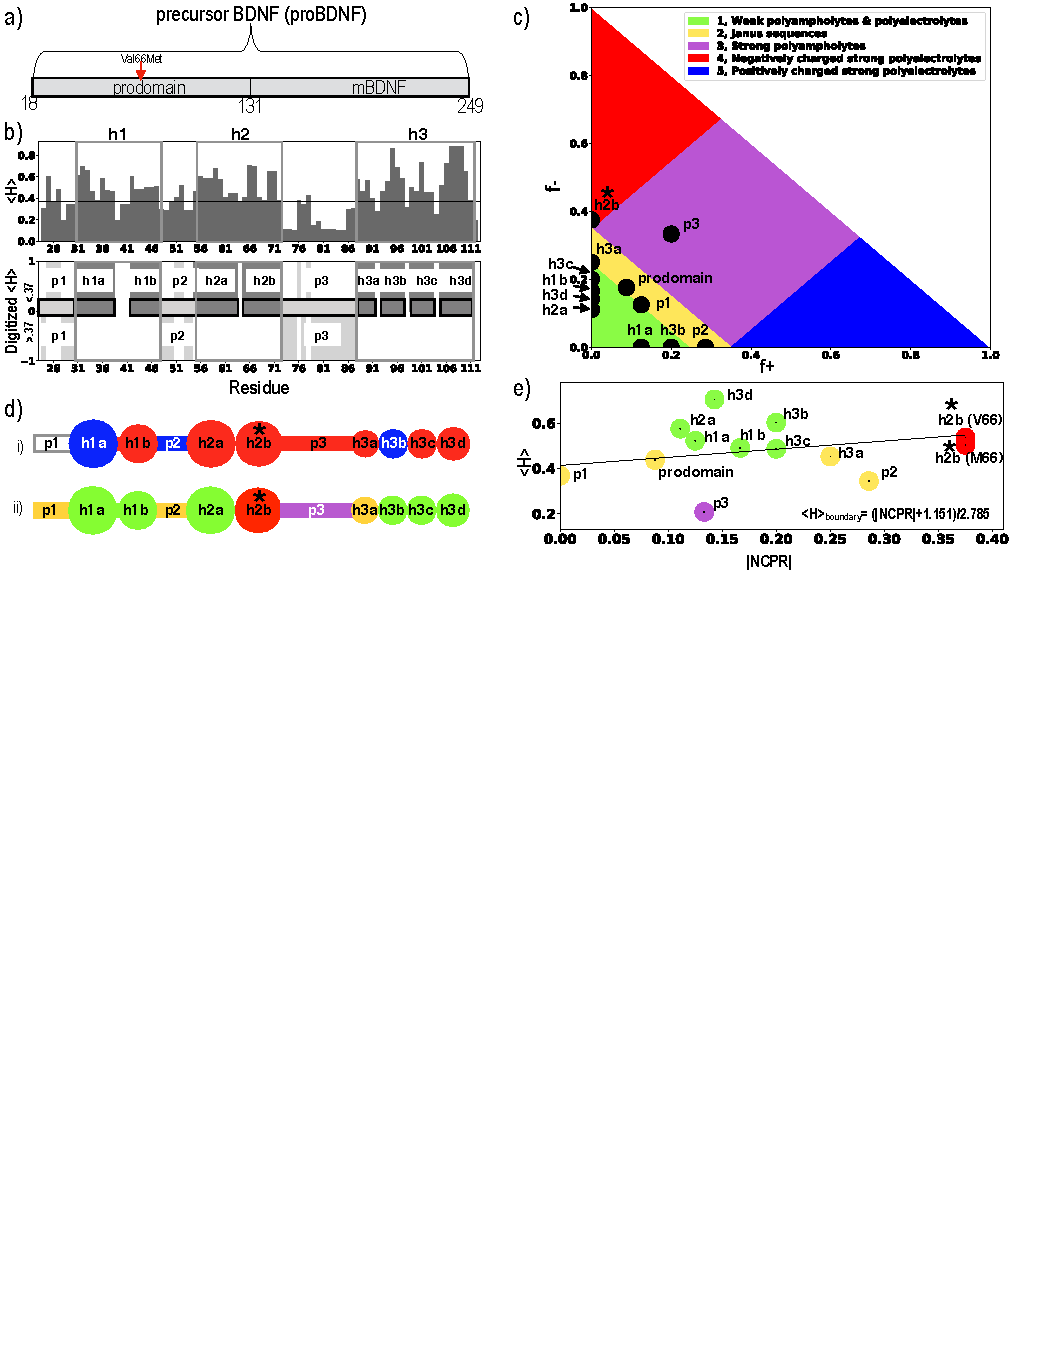
\includegraphics[scale=0.5,width=\textwidth,trim={0 0cm 0 0cm},clip]{../figures/fig1.pdf}
\caption{{\bf Electrostatics in the IDP diagram of states and proBDNF prodomain.} 
a) Diagram of states reported by Ref.~\cite {Das2015,Das2013a}, based on fraction of positively and negatively-charged residues.  As indicated, the V/M66 BDNF prodomain lies on the boundary between the Janus region and the weak polyampholyte/polyelectrolyte regime. b) proBDNF consists of two domains: the prodomain and mature BDNF (mBDNF). %We simulated prodomain residues 23-113 for both V66 and M66. 
c) Mean hydrophobicity and net charge per residue (NCPR) for the prodomain, based on a sliding window of 5 residues, showing a positively-charged N-terminal region, negatively-charged C-terminal region and a hydrophobic and highly negatively-charged mid-sequence region (containing the Val66Met SNP). Parts a) is generated with CIDER. ~\cite {Holehouse2017} }
\label{fig1} 
\end{figure}


Difficulties in obtaining unambiguous disease associations at the proBDNF Val66Met SNP using GWAS are paralleled by challenges in characterizing its effects on the properties of the BDNF prodomain using structural techniques.  A crystal structure of a homologous neurotrophic factor in complex with a shared receptor, revealed a well-defined volume corresponding to the prodomain, but which lacked resolvable density.\cite{Feng2010a} 

It was subsequently revealed that the cleaved prodomains ($\sim90$ residues) are found in monomeric states {\it in vivo}, and the M66 (but not V66) form binds to SorCS2 (sortilin-related VPS10p domain containing receptor 2), leading to axonal growth cone retraction.\cite{Anastasia2013} NMR measurements on the prodomain confirmed significant intrinsic disorder for both forms, with differential secondary structure preference around residue 66. ~\cite {Anastasia2013}.  It was not possible to gain any insight into the BDNF prodomain tertiary ``structure'', with uncertainty in interpretation of NMR signal obscuring whether secondary structure is affected far from the SNP, but additional NMR experiments implicated residue 66 in binding of M66 prodomain 
 to SorCS2.~\cite {Anastasia2013}
 
The Val66Met is present in a region with high density of negative charged residues (D61,E64,E68,E69). In this scenario, residue his65 can exist in protonated or neutral charge state in vivo due to it's low pKa. In order to capture the effects of histidine protonation states on Val66Met, we study the Val66 and M66 prodomain in presence of both neutral His65 and protonated His65.

In this work, we report on unbiased fully-atomistic replica-exchange MD simulations of the 90 residue BDNF prodomain in explicit solvent, for V66,   V66\textsuperscript{65+}, M66 and  M66\textsuperscript{65+} forms.  This sequence falls at the boundary of the Janus and globular domains in the diagram proposed by Das and Pappu. \cite{Das2015,Das2013a} 


%and exhibits sufficiently fast kinetics that %we were able to use a relatively narrow temperature range and small number of replicas; the overall calculation required an expensive, but feasible, 78 $\mu$s of simulation.  
%We measure secondary structure tendencies consistent with NMR data, and show that differential helical tendencies are consistent with increased entropic cost of the valine side-chain in a helix conformation.  We develop a tractable framework for interpreting transient tertiary contacts, allowing us to identify about 12 regular pairing sites along the BDNF prodomain  sequence, which are stretches of the protein several residues long with an elevated tendency to form $\beta$ bridges.  Most significantly, we find that the backbone conformation local to residue 66 can predict such pairings.  The charge-neutral Val66Met SNP is observed to affect the loose tertiary ``structure'' of BDNF prodomain by altering the local secondary structure of the adjacent highly charged region, which in turn affects long-range interactions between distant residues.  




% Results and Discussion can be combined.
\section*{Results and Discussion}

\subsubsection*{Selection of force field}
In order to get accurate structural characterization of proBDNF with MD,  we did  500ns of T-REMD simulations of 30 residue fragment of V66 proBDNF with few popular ff and water model combinations and proceed with the one which gave best agreement with experimental data obtained by NMR. Fig~\ref{fig2}a compares the CA shifts for  Amber99sb*-ildn-q with Tip4p-D,  Amber99sbws, Amberff03sbws, Amber99sb-ildn with Tip3P and NMR.  Amber99sb-ildn with Tip4p-D and Amber99sbws gives good agreement with NMR CA chemical shift.  We also compared Rg distribution for the tested ff (Fig~\ref{fig2}b).  Tip3P generates very collapsed ensembles and the remaining three ff generates similar Rg distribution. Tip3P is known to produce structures which are too collapsed relative to experiment. Since, the remaining three ff gives comparable Rg, we proceed with Amber99sb*-ildn-q with Tip4p-D because it gives the best match with experiments. 

 \begin{figure}[!ht]
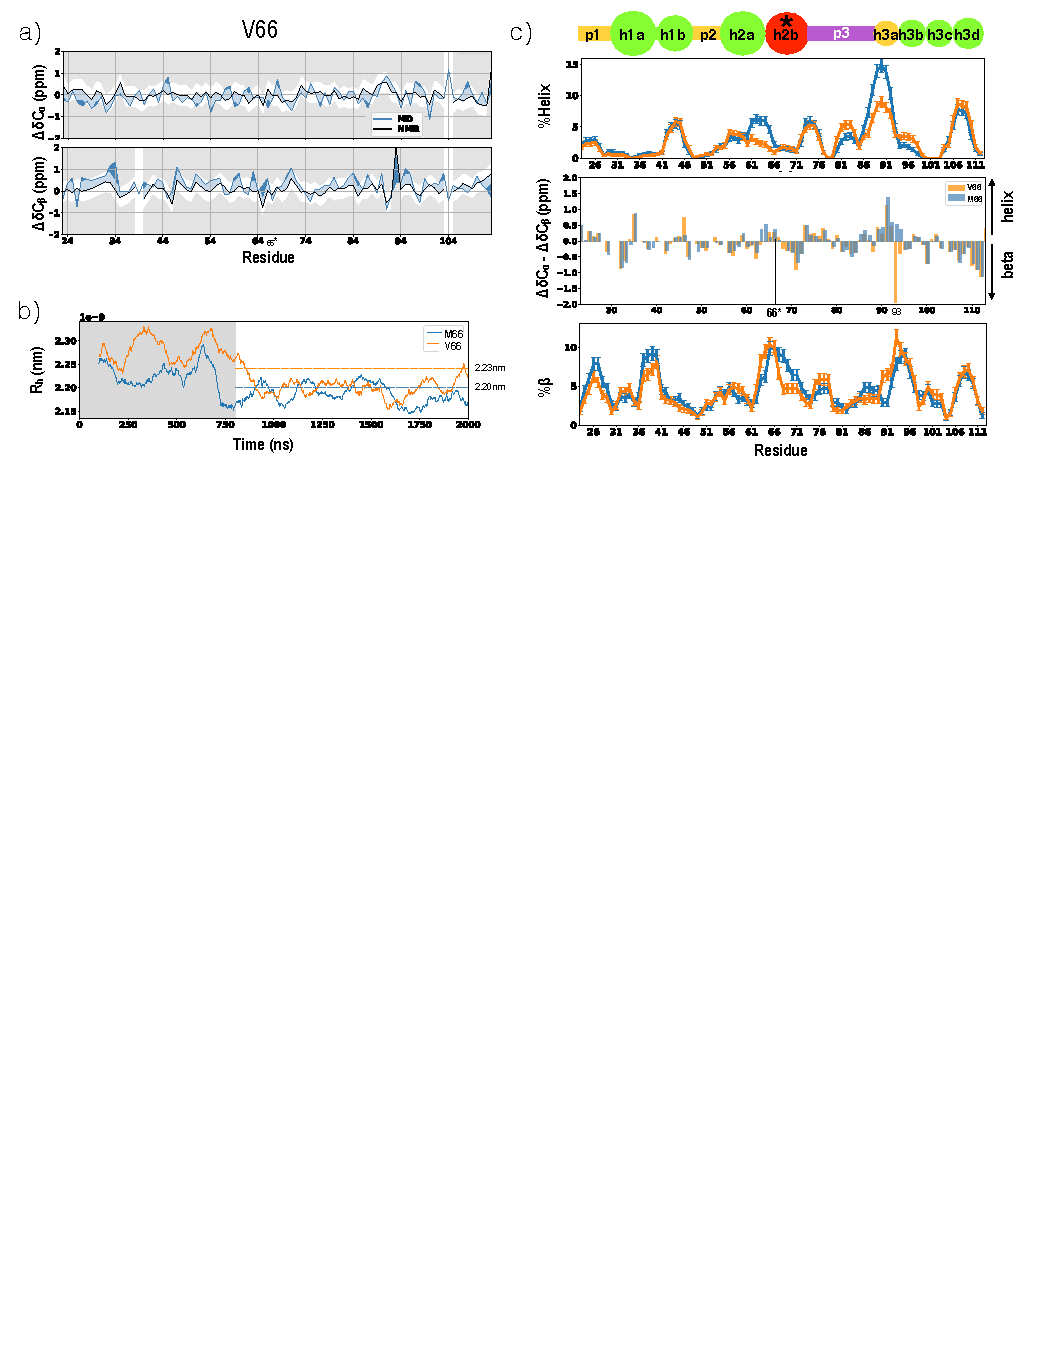
\includegraphics[scale=0.5,width=\textwidth,trim={0 0cm 0 0cm},clip]{../figures/fig2.pdf}
\caption{{\bf Ff comparison.} (a) Comparison of calculated chemical shifts from MD ensembles at 280K and NMR chemical shifts from ~\cite{Anastasia2013}  at 280K,  as described in methods. (b) Rg distribution for each ff.}
\label{fig2} 
\end{figure}

\subsubsection*{Predictions from MD trajectories {\it vs} NMR data} 

In order to access the validity of MD generated ensembles, we compare the MD ensembles with experimental data obtained by NMR spectroscopy and NMR diffusion measurements. Fig~\ref{fig3}a compares MD chemical shift and NMR chemical shifts. We get good agreement with NMR chemical shifts; deviations at each residue is \textless 0.5 ppm. Although there are some localized discrepancies for certain residue types, we get discrepancy at same residues for all four simulations. Thus, specific discrepancy is probably reflecting residual force-field inaccuracies. Consistent with intrinsic disorder, helix and $\beta$ propensity for each residue was low for both MD at 300K and NMR data at 280K. The simulated hydrodynamic radii (calculated using hydropro) of V66 (2.21 nm) and M66 (2.18 nm) are in excellent agreement with the experimental values (2.24 nm and 2.20 nm respectively) (Fig~\ref{fig3}b). This, confirms that the overall dimensions of the proteins is reasonable.

\subsubsection*{Our simulations are well converged} 

Most of the IDP simulations studies have been performed on smaller IDP fragments (residues 3-40). We performed the explicit solvent replica simulations of 91 residues, which was computationally challenging and thus we carefully accessed the convergence of our simulations. All replicas were able to diffuse in the temperature range 300K to 385K (replica round trip number \textgreater 7) (Fig S1). The Rg for V66 and M66 converge after 800ns of simulation at 300K (Fig~\ref{fig3}b). We discarded the first 800 ns of the trajectories as conformational equilibration. The Rg distribution of all four simulations are symmetric/unimodal (Fig~\ref{fig3}c). Mostly, asymmetric form of Rg distribution has found to be indicative of lack of convergence. 

\begin{figure}[!ht]
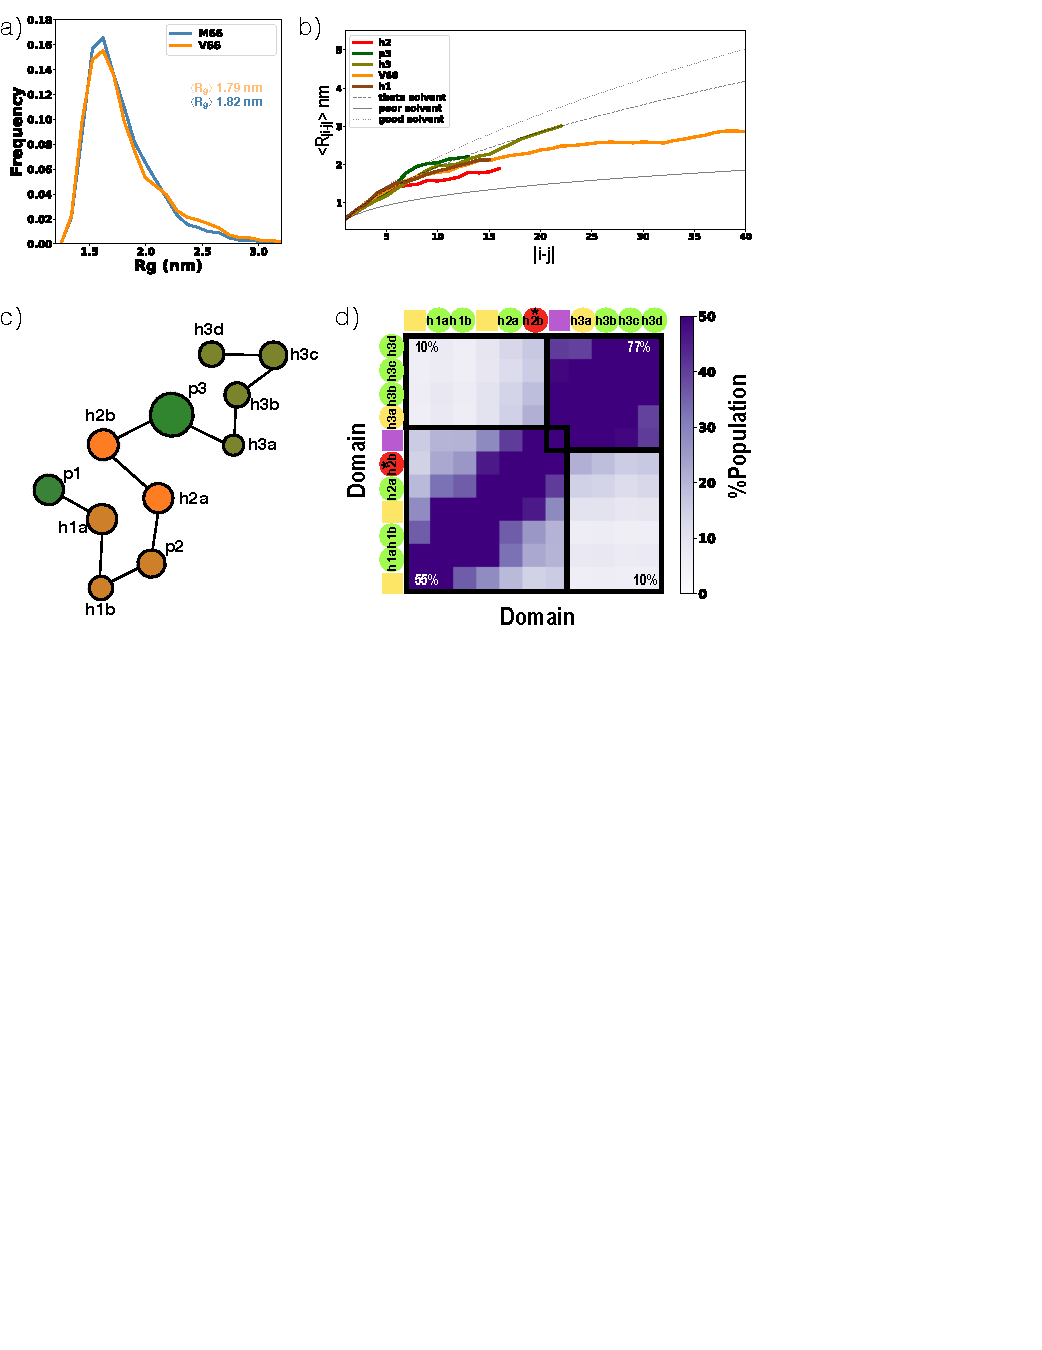
\includegraphics[scale=0.5,width=\textwidth,trim={0 0cm 0 0cm},clip]{../figures/fig3.pdf}
\caption{{\bf Comparison of MD and NMR observables.} a) Comparison of calculated chemical shifts from MD ensembles at 300K and NMR chemical shifts from ~\cite{Anastasia2013}  at 280K,  as described in methods. b) Rh at 100 ns moving  window for V66\textsuperscript{65+} and M66\textsuperscript{65+} vs simulation time. The Rh for V66\textsuperscript{65+} and M66\textsuperscript{65+} converge after 800ns of simulation at 300K. c) Rg distribution for each simulation }
\label{fig3} 
\end{figure}


\subsection*{Val66Met changes local and non-local secondary structure}

\textbf{Both mutation at residue 66 and protonation at 65 increases helix formation at residue 66.} 
NMR studies found differential chemical shifts at residues 66 and 93 ( marked with stars ) for Val66Met (Fig~\ref{fig4}a). Consistent with NMR data, both Val66Met and Val\textsuperscript{65+}66Met\textsuperscript{65+} changes the frequency of long helix ( \textgreater 6 residues)  formed at residue 63 and 93 and beta sheets ( \textgreater 4 residues) at residue 93  (Fig~\ref{fig4}b). However, how the mutation causes this differential chemical shifts is not known. 
To look into the effect of mutation on residual secondary structure, we compare the helix tendency at every residue for each of the four simulation (Fig~\ref{fig4}c). M66 and M66\textsuperscript{65+} has increased tendency of forming $\alpha$-helix at residue 66 when compared with V66 and V66\textsuperscript{65+}(Fig~\ref{fig3}b). To get more insight at the helix formed at 66, we look at the population of each helix length formed at 66 (Fig~\ref{fig4}d). Only M66 and not V66 has long helix formation at residues 59-67 (9 residues). Additionally, M66\textsuperscript{65+} forms even longer helix 62- 71 (10 residues) . Increased helix formations in M form is consistent with earlier observation, where an increased entropic cost of helical formation for the valine side-chain, which can access only one of three possible side-chain conformations \cite{Creamer1992}. Protonated histidine favors longer helical structure at residue 66 due to helix favored salt-bridge formation  Glu61\textsuperscript{65+} and Hip65-GLU69. 

We also look at the temperature dependence of helical structure in prodomain. At 385K, the helix at residue 66 increases (\textgreater 2\%) for all V66, M66, V66\textsuperscript{65+}, but M66\textsuperscript{65+} has strongest preference (\textgreater 5\%) (Fig~\ref{fig4}c). 

\textbf{Only Val66 and not Met66 forms long beta sheet structures at residue 66 and 93.} We next examined the backbone contacts formed between residues.
% Hip65 reduces beta sheet tendency at residue 66 for both V and M form (Fig~\ref{fig5}a). This could be due to gain of helix at 66 in Hip65 form or due to loss of sheet structures which involved salt-bridge formation at 64. 
V66 and M66 forms differential backbone contact at residue 66 (Fig~\ref{fig5}a). V66 forms beta sheet structures with residue 92. This is also consistent with NMR observation, where Val66Met changes CS at residue 93 (Fig~\ref{fig4}a) . 
We further test if the beta sheet structures at residue 66-95 in V66 is more favored in V66 than in M66 and is not a limitation of simulation convergence. To verify this observation, we performed simulations with backbone restraints of 1Kj/mole/nm2 of a V66 frame having beta sheet structures at residue 66-95 with Val66 mutated to Met. We find that M66 has higher loss in entropy at 93 (Fig~\ref{fig5}b). Additionally, 66-92 beta structures forms 64-93 salt bridge simultaneously in V66(Fig~\ref{fig5}c). In our restrained simulations M66 has 50\% less probability of forming salt-bridge at residue 64-93 (Fig~\ref{fig5}d). This result suggests that beta at 66-95 is less favored in M66 due to higher entropic and energetic cost. 

%We also look at the temperature dependence of  $\beta$ structure in prodomain. At 385K, the $\beta$ at residue 66 decreases for all four simulations V66, M66, V66\textsuperscript{65+} and M66\textsuperscript{65+}, however V66 has strongest preference of $\beta$ at 66 (\textgreater 2.5\%) (Fig~\ref{fig4}c). This further suggests that $\beta$ at V66 is more favored than M66 due to lower entropic cost of forming $\beta$ strands.

\textbf{M66 supports helix formation at residue 93}

We next examined the increased helix tendency at residue 93 from Val66Met substitution. We find structures forming helix at 93 are in contact with residue 66 in at-least 25\% of it's population in M66\textsuperscript{65+} (Fig~\ref{fig6}). The gain of this residue specific interaction in M66, probably increases helix formation at 93 when compared with V66. 

\begin{figure}[!ht]
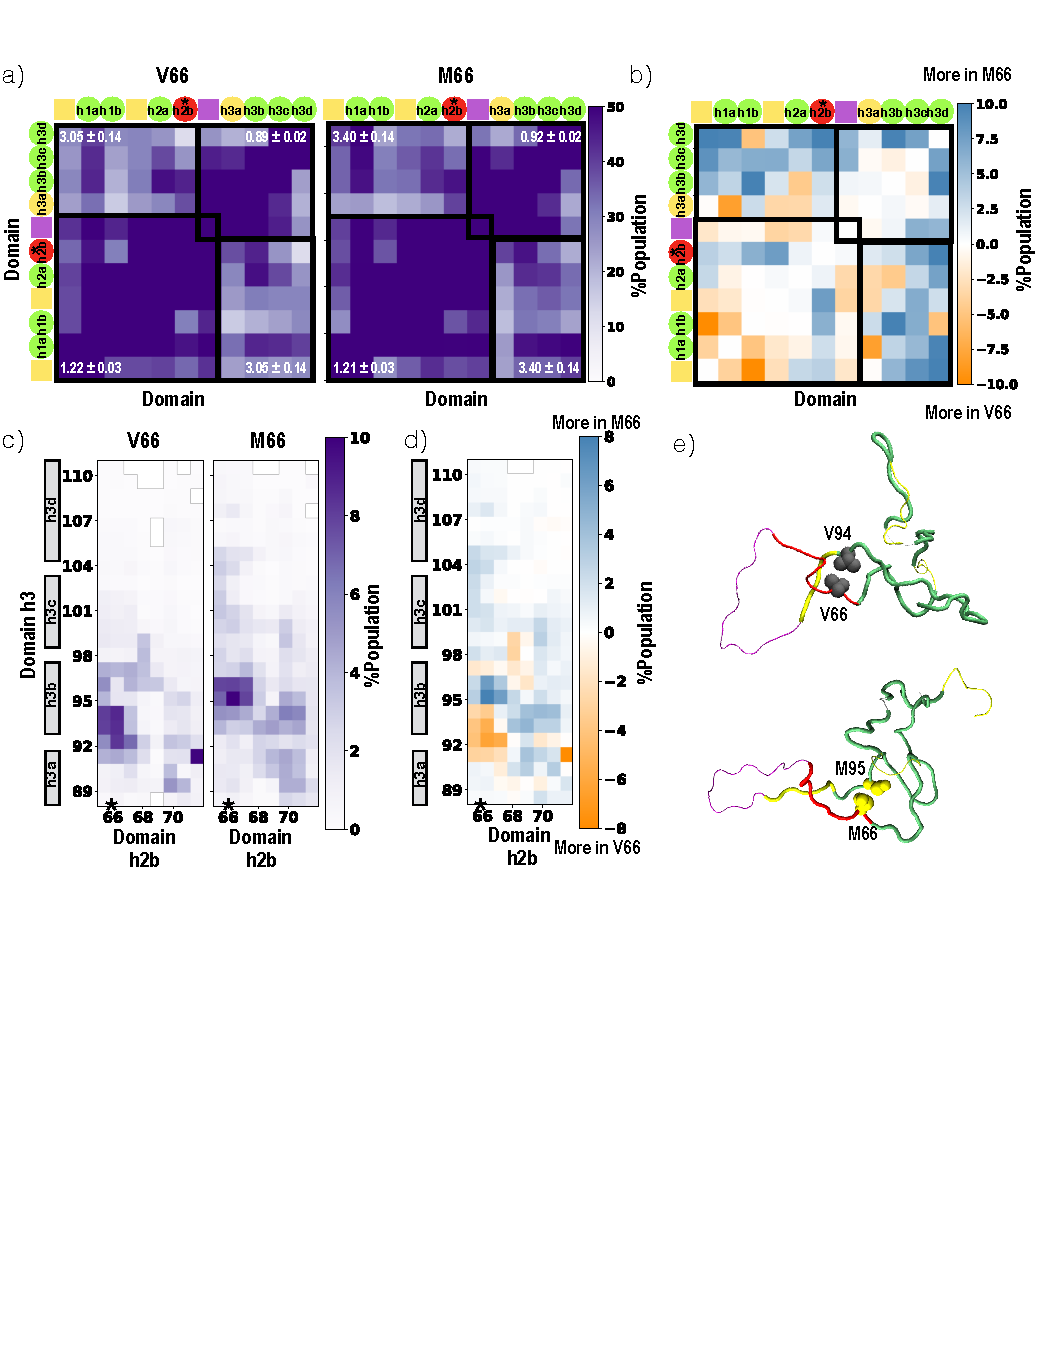
\includegraphics[scale=0.5,width=\textwidth,trim={0 0cm 0 0cm},clip]{../figures/fig4.pdf}

\caption{{\bf Simulation predicted helical structure and it's comparison with experiments.}
a) CA-CB secondary chemical shifts for V66 and M66 from  ~\cite{Anastasia2013}  at 280K. Positive difference indicate helical structure and negative differences indicate beta structure. Residues 63-67 and residues 93-95 have slightly higher tendency of being helical in M66 ( marked with stars ). b) Difference in helix length (top) and beta length (bottom) for each residue. In agreement with the experiment, we find higher tendency of forming longer helix at the regions marked with stars. V66 has higher tendency of forming beta at residue 93. c) STRIDE predicted secondary structure at each residue at 300K (top) and 385K (bottom).  Protonated his65 has increased tendency of forming long helix at residue 66 only for M66. The background of the plots are colored according to residue type: blue-basic, red-acidic, green-polar, white-hydrophobic. d) Helix length distribution at each residue when 66 is in the helix region of ramachandran map (methods) }

\label{fig4} 
\end{figure}


\begin{figure}[!ht]
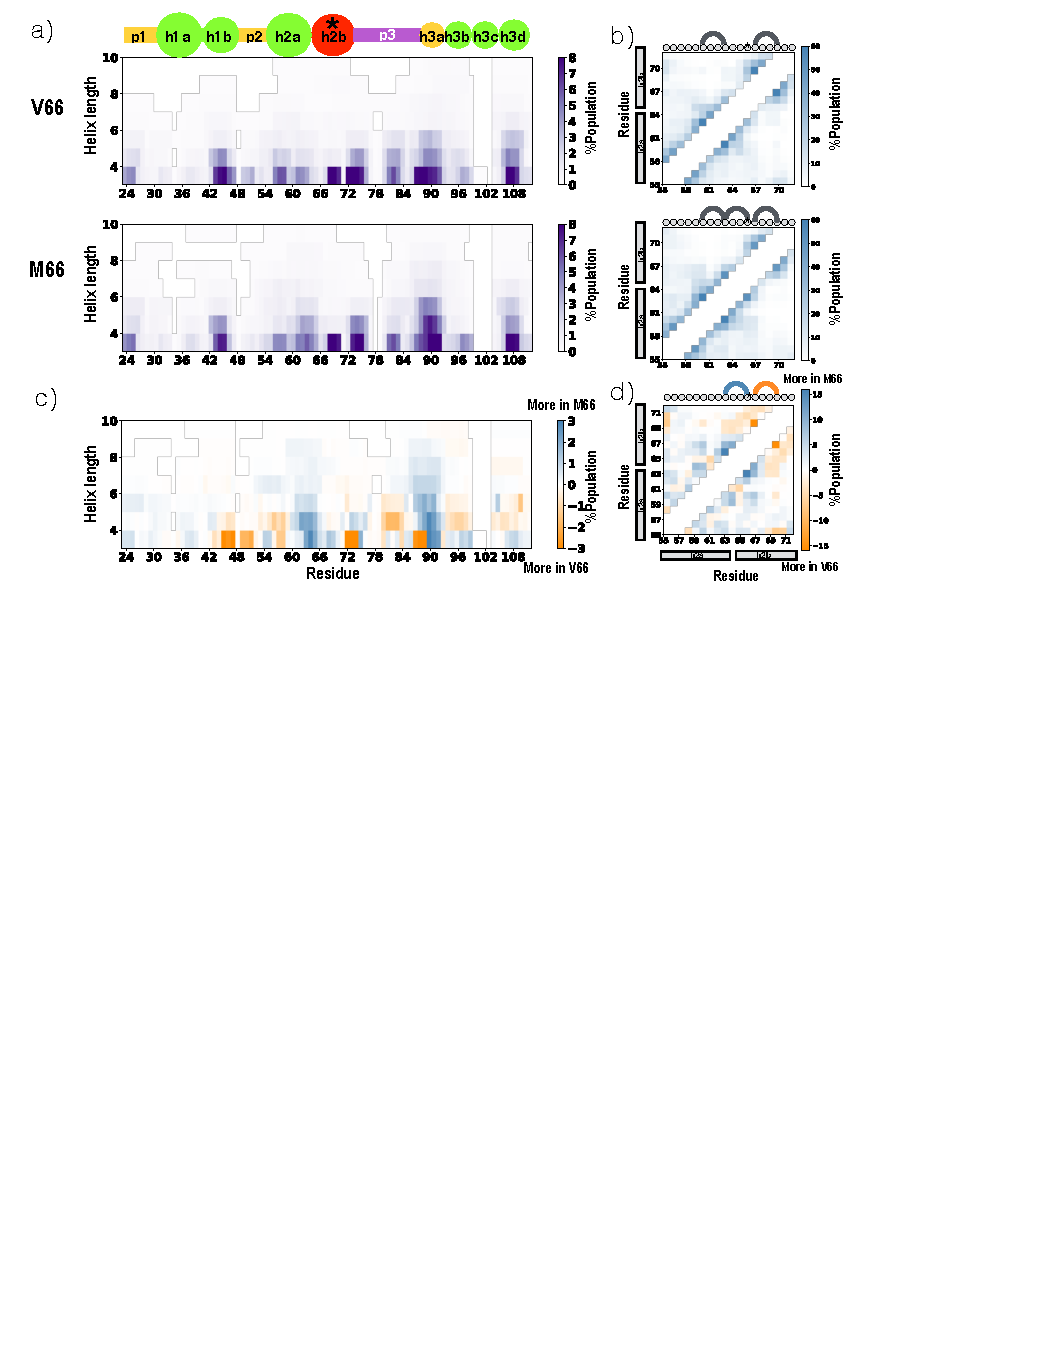
\includegraphics[scale=0.5,width=\textwidth,trim={0 0cm 0 0cm},clip]{../figures/fig5.pdf}

\caption{{\bf Backbone contacts at residue 66.}
A) Difference in V66 and M66 backbone contacts. Contact difference \textgreater  5\% are also shown with network representation. b) Change in entropy at every residue from random coil when 66-95 are in beta sheet structures. c) VMD representation of a V66 frame when 66 and 95 forms backbone h-bond. d) Population of salt bridge formed at 64-93 when 66 is in beta sheet structure with 92.   
}


\label{fig5} 
\end{figure}

\begin{figure}[!ht]
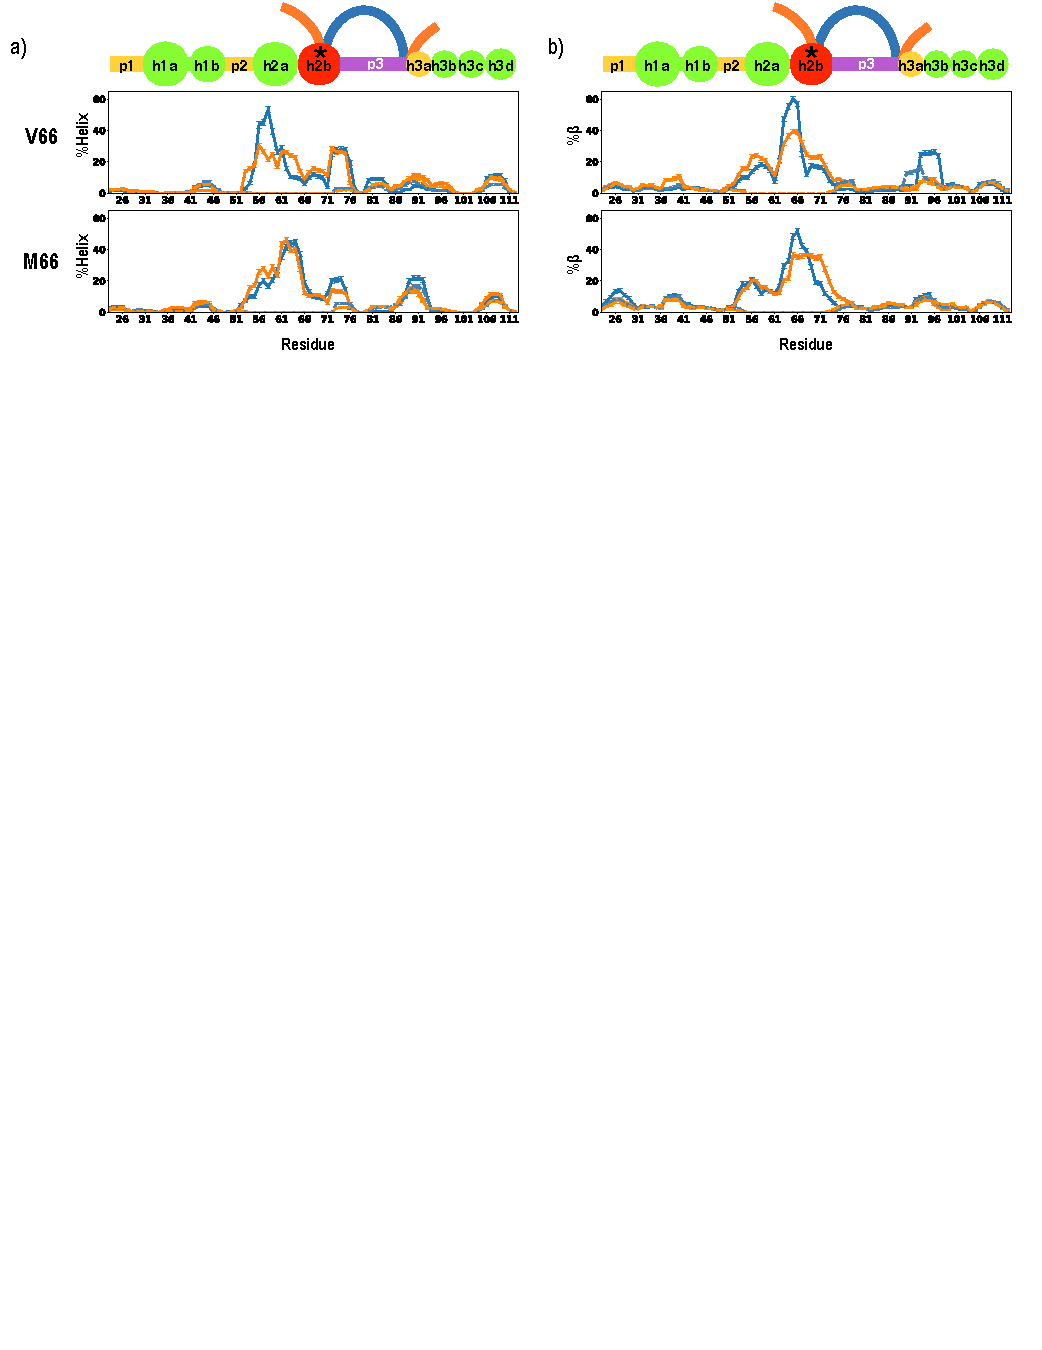
\includegraphics[scale=0.1,width=12cm,trim={0 0cm 0 0cm},clip]{../figures/fig6.pdf}
\caption{{\bf M66 supports helix formation at residue 93 } 
a) Backbone tertiary-contact network for M66\textsuperscript{65+} when 93 is in helix. Met66 stabilizes the helix formed at residue 93. b) VMD representation of a frame forming helix at 93 and contact at 66-93. 66 and 93 are shown in vanderwaal representation with grey and magenta color respectively.}
\label{fig6}
\end{figure}



\subsubsection*{Long range contacts involve residue 66 or the termini} 

Conventional contact maps provided little useful insight into tertiary structure for either forms of the protein, which was consistent with the intrinsic disorder and frequent transient interactions among neutral side-chains. Identification of contact residues yielded several persistent, weak long-range interactions at 300K for both sequences, which can be represented along a single axis (Fig~\ref{fig6}). 

Prodomain has well defined regions forming long-range tertiary contacts. From the tertiary contact maps from all four simulations, three regions are identified which forms high density of long range contacts; -1': residues 31 to 35, 0': residues 57 to 69, +1':  94-98 and +2': 106-109 (Fig~\ref{fig6}). All the three regions identified has high density of hydrophobic residues (Fig~\ref{fig7}a). It has been frequently observed that unfolded proteins form strong hydrophobic contacts. Thus, it's not very surprising that the disordered prodomain has the presence of strong hydrophobic contacts. Charges in the hydrophobic regions seem to determine the strength of contact formed between two hydrophobic regions.  0' region, which is negatively charged forms contact with positively charged +1' region or neutral -1' region. 


\textbf{Effects of H65 protonation states on long range tertiary contacts.} These contact maps for the entire ensemble indicate far more tertiary contacts between the sequence midpoint and the terminal domain of the sequence for V66 and M66 when compared with the protonated H65. Hip65 looses long range contacts for both V66 and M66. It has been earlier observed that fraction and distribution of charged residues along the disordered protein sequence determines the long range contacts. Several residues near the mutation (residues E64,E68, and E69) are negatively charged. Both V66 and M66 looses salt-bridge with the gain of positive charged residue in the otherwise negatively changed region of the sequence. 

\textbf{V66 collapse is driven by electrostatic contacts at center whereas M66 collapse is driven by hydrophobic contacts.} We look at the effect of Val66Met on long-range contacts. Even though the prodomain is disordered we identify loss of specific residue contact at 66. M66 and M66\textsuperscript{65+} forms strong hydrophobic contacts at residue M66-Y34 when compared with V66 and V66\textsuperscript{65+} respectively.  
In V66, Y34 forms strong contact with residue L70. However, this hydrophobic contact is formed with simultaneous salt bridge formation between residue 27 and 72. 
The strong hydrophobic contacts at residue 66 forms comparatively collapsed structures in M66, M66 (p) when compared with V66 and V66 (p). 



%\subsubsection{Local contacts at residue 66 modulate long range contacts}
%Val66Met has increased helicity at residues 63-66 due to gain of helix forming hydrogen-bond 63-67 and 62-66. Frames forming helix at residue 66 is less likely to form other long range-contacts. Frames with helix at residue 93 have contact formation at 66-93(Fig ~\ref{fig5}d). 

%Frames forming beta-sheets at 66 have higher tendency of forming long range contacts. For V66 67-71 and 65-92 together forms beta sheet structures. 


%Hip65 gains further strength for helix formation at residues 63-67 due to gain of positive charge at the otherwise negatively charged region. 




%\subsubsection*{V66M looses long-range contact at residue 66} 


%V66 forms beta sheet at residue 66 with residue 92. These beta-sheet structures also form salt bridge at residue Glu64 and Arg93.

%Three regions 33-34, 92-95, 63-66, 67-70 are hotspot regions for forming long extended beta sheet structures. When residues from the midpoint  form contatcts with the center region, we get compact structures. 
%63-66 is involved in backbone h-bonding, in V66 66 forms long range contacts with 93.

%In His65 protonated these contacts are lost due to the protonation state of histidine. Thus, charged histidine conformers loose the salt-briding with the other 93 residue. 70 looses helix structure. 

%\textbf{show the histogram plot for protonated and non-protonated histidine.} 

%\subsubsection*{V66M forms more expanded ensembles than M66 in protonated form}
%\textbf{Look at why we have have co-operative helix formation at residue 66 and 93 ? is it just in the protonated form. Identify these replicas and look at them in vmd.}





\begin{figure}[!ht]
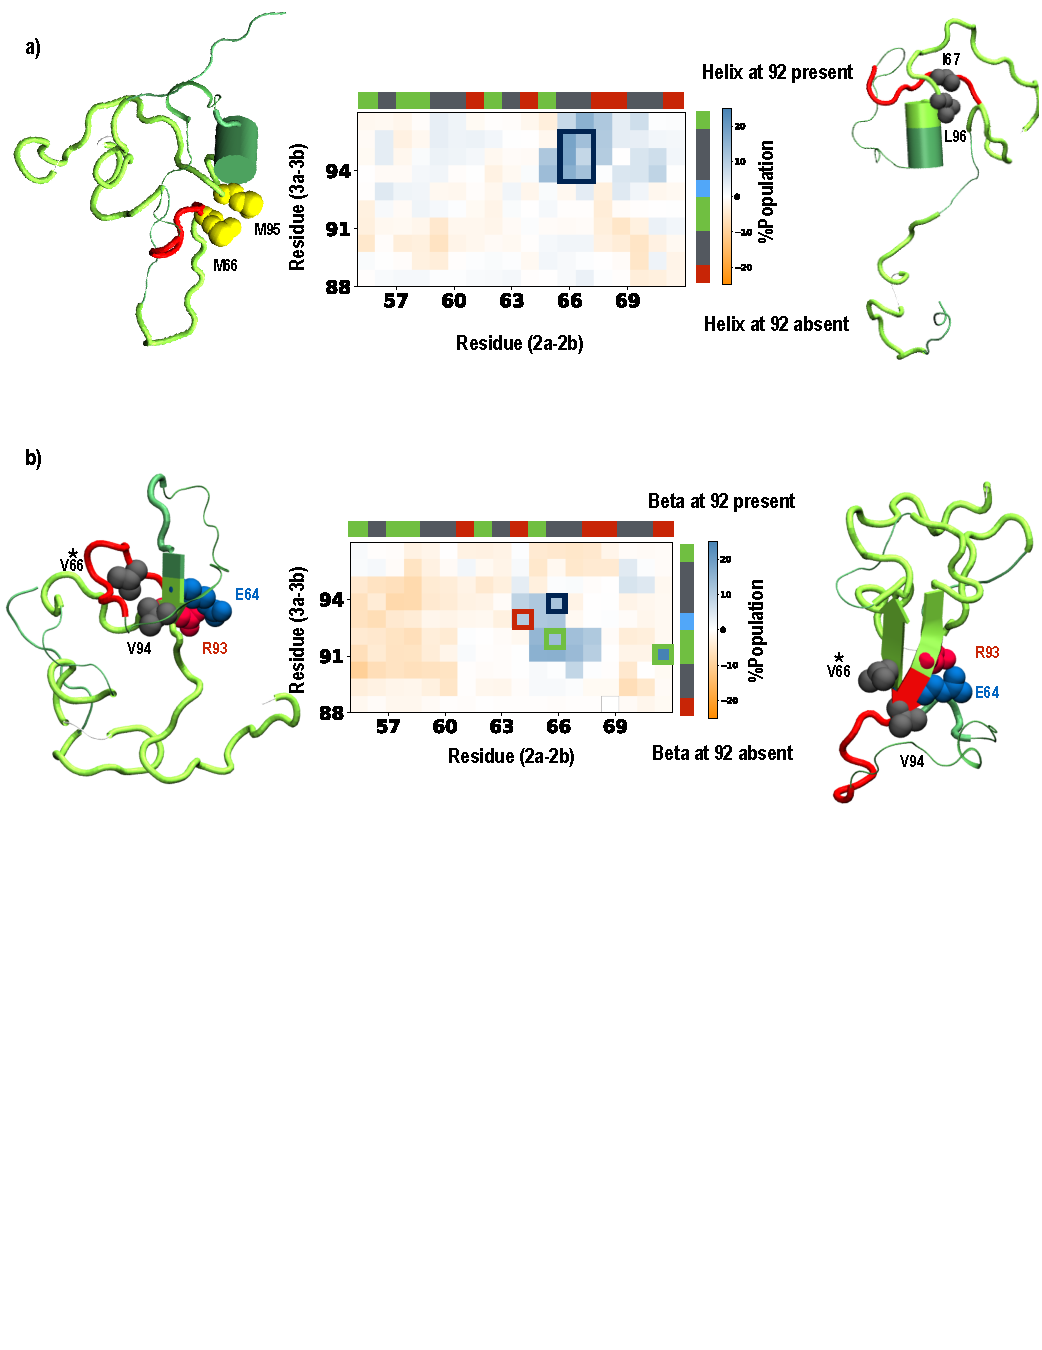
\includegraphics[scale=0.5,width=12cm,trim={0 0cm 0 0cm},clip]{../figures/fig8.pdf}
\caption{{\bf Linear networks of transient tertiary contacts.} a) The backbone tertiary-contact network is made for V66 and M66, with each residue serving as a node in the network, as described in Methods. A contact is formed if two residues are within .45nm of each other. If the two residues forming contact are more than 24 residues apart the edge is drawn on the top of the node, otherwise the edge is drawn at the bottom of the node. Backbone interactions serve as edges between individual network nodes; the thickness  and the transparency of the edge corresponds to the strength of the contact. Contacts observed in 37 or more replicas are only visible.  Gain of protonation states looses contacts formed from 0' region for both V66 and M66. V66 to M66 gains contact at residue 66-34 for both neutral and protonated histidine at residue 65. b) Internal residue level scaling for each peptide.
 }
\label{fig8}
\end{figure}


\begin{figure}[!ht]
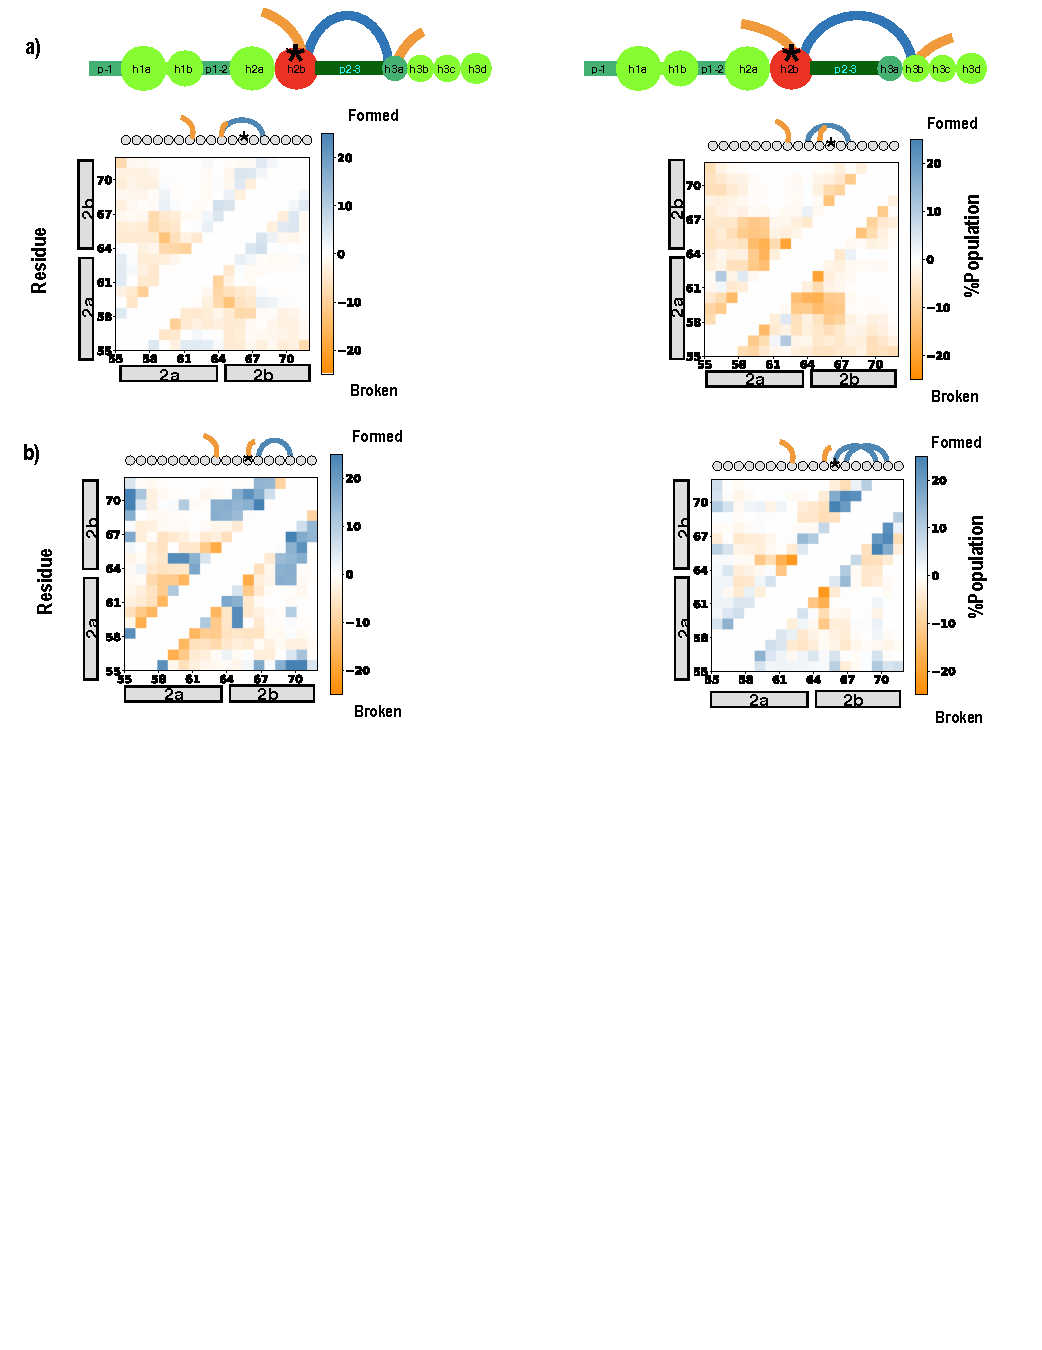
\includegraphics[scale=0.5,width=12cm,trim={0 0cm 0 0cm},clip]{../figures/fig9.pdf}
\caption{{\bf Long range contacts are correlated with short range contact at residues 63, 65, 66 or 67, 69.} Two strongest non-correlated long range contact formed in V66 a) and M66 b). 
 }
\label{fig9}
\end{figure}
\section*{Conclusion}

We have carried out ~.5ms of fully-atomistic MD simulation of the 90 residue prodomain of brain-derived neurotrophic factor with protonated and neutral His65 state, for both with and without the disease-associated Val66Met mutation.  

Anastasia et al~\cite{Anastasia2013} observed differential kinetics for interactions between BDNF prodomain and SorCS2; M66 binds more strongly at residues H65 to L71 with SorCS2, whereas V66 binds more strongly at residue Y90 to V94. 
The stronger binding at residue M66 could be attributed to either a) ability of M66 to form alpha-helix at residue 66 when compared with V66 or b) stronger hydrophobic contact at residue M66 with the SorCS2 hydrophobic residues or combination of both a) and b). 

Residue 66 possess several meaningful properties, beyond including the disease-associated mutation of our original interest. It is a) neutral residues inserted in a stretch of acidic residues constituting the most highly charged region of the protein and b) directly adjacent to the sequence midpoint at E68.  We have not yet isolated which of these contribute to the critical role of residue 66 in forming strong tertiary interactions, and it is possible that overlap of (a) with (b) is intrinsic to the protein design.  


%\subsection*{V66 and M66 has differential secondary structure and reverse secondary structure trends }

%\subsubsection*{Sensitivity of predictions to algorithm}


%d2D was used to reanalyze the chemical shift data from\cite{Anastasia2013} as described in methods, and indicated significant PPII tendency in BDNF prodomain 
 %for both V66 and M66 forms (Fig~\ref{fig2}a). Both TALOS+ and d2D indicated significantly higher $\beta$ propensity in V66 at regions 0\textsuperscript{$\prime$} and +1\textsuperscript{$\prime$} relative to M66 (Fig~\ref{fig2}b). Unlike TALOS+ predictions, d2D also predicts higher $\beta$ at region +4\textsuperscript{$\prime$} for V66.  This may reflect the simplest scenario involving secondary structure coupling: reducing $\beta$ propensity at one residue automatically reduces $\beta$ propensity for any $\beta$ bridging partners of that residue.  (In the MD simulations, we do observe the 0\textsuperscript{$\prime$} and/or +1\textsuperscript{$\prime$}  pairing with +4\textsuperscript{$\prime$} in the V66 form, an interaction likely stabilized by the negative charge in the +1\textsuperscript{$\prime$} region interacting favorably with the positive charge of the +4\textsuperscript{$\prime$} region in the BXH cluster, which is likely to be even more populated at the colder temperature used for the NMR data. ) 


%\textbf{Comparison of STRIDE and d2D secondary structure predictions in MD generated ensemble}. 
%As shown in Fig~\ref{fig2}d, some conformations will be identified as indicating $\beta$ structure by d2D but not by STRIDE; in general, these are conformations in which the backbone is consistent with a $\beta$ conformation, but has no partnering strand.  Conversely, for some residues STRIDE identified $\beta$ structure while d2D did not; this is most striking at the neutral stretch of residues around +4\textsuperscript{$\prime$}, where d2D predicts $\beta$ structure from NMR chemical shifts and STRIDE predicts $\beta$ structure from MD coordinates, but d2D does {\emph not} identify significant $\beta$ structure from the MD-generated chemical shifts. 


%, with discrepancies indicating slightly reduced secondary structure in the MD simulations, consistent with simple expectations based on the higher temperature used. 
% although we observe less PPII and beta tendency at several residues in MD ensembles when compared with NMR. For most of the residues, an increase in replica temperature corresponds with loss of beta structure, indicating the increased $\beta$ tendency for the NMR data may reflect the reduced temperature (280K), particularly in the region around the SNP ($-1^\prime$,$0^\prime$,$+1^\prime$)  for V66. 
%For a few regions of the prodomain (regions $-3^\prime$ and $-4^\prime$ for both V66 and M66), MD simulation slightly underestimates PPII (and overestimates coil) propensities.  MD simulations also suggest a helical C-terminus (at $6\textsuperscript{$\prime$}$) for both V66 and M66 sequences, while this region is highly disordered according to interpretations from NMR. This discrepancy is not consistent with a simple temperature effect, according to the observed temperature trends, but may reflect differences in terminal interactions, including potential interprotein interactions within the experimental system. 
%It is 

%Discrepancies are unlikely to simply reflect poor convergence of the MD data, since trends for different temperatures were smooth, and all replicas were able to diffuse in the temperature range 300K to 420K (\nameref{S1_Fig}).
  

% Through extensive decomposition of the resulting ensembles, we find that the backbone configuration around residue 66 adopts several configurations at 300K, each of which is associated with a particular set of long-range contacts, summarized in Fig~\ref{fig8}.

%\begin{figure}[!ht]
 %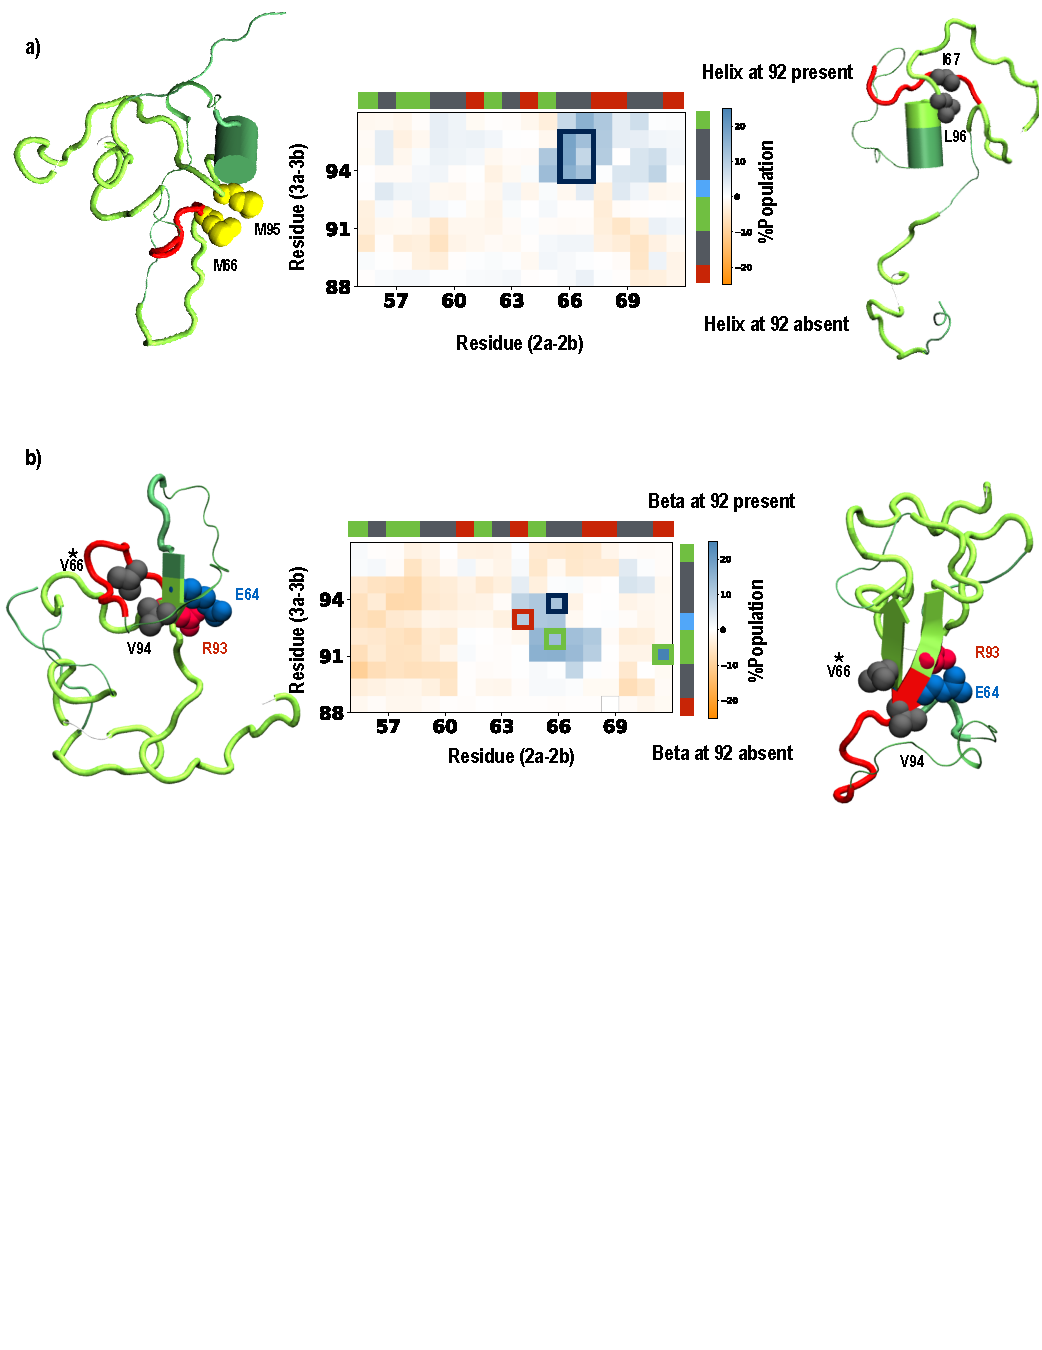
\includegraphics[width=8cm]{../figures/fig8.pdf}
%\caption{{\bf Proposed mechanism for modulation of tertiary contacts via local conformation around residue 66.}
%Blue circles and red circles indicate pairing regions in positively and negatively charged regions, respectively; residue 66 (0\textsuperscript{$\prime$}) is indicated by a hollow black circle.  Common long-range contacts are shown as solid lines, with possible sequence-dependent contacts shown as dashed lines (V66 in black, M66 in green).   Orange symbols represent helical stretches (rectangles) or forced helical breaks (lines), corresponding to the associated cluster in the right column.  Cluster XHB shifts the helical break in the C-terminal direction from its location in cluster BXH, allowing increased backbone pairing within the C-terminal side but decoupling it from the N-terminal side.  
%}
%\label{fig8} 
%\end{figure}

%The origin of this difference was determined using the clustering process outlined previously. Diagrams of each the ordered clusters (BBB and HHH) reveal similar patterns for V and M within each cluster; for these clusters, tertiary contacts are much more sensitive to the backbone conformation at residues 65-67 than to whether residue 66 has a side-chain of V or M.  It is challenging to test the same claim for disordered clusters, because the disordered clusters are each sparsely populated in either V66 or M66 at 300K; e.g. XHB and BXH do not contribute significantly to the V66 and M66 ensembles respectively, but are the most populated cluster for M66 and V66 respectively.  




%The average radius of gyration R\textsubscript{g} indicates an ensemble of more compact conformations for the V66 sequence at 300K; R\textsubscript{g} = 1.35 $\pm$ .01 nm and 1.39 $\pm$ .01 nm for V66 and M66 respectively. We observe a reversal of the temperature dependence in R\textsubscript{g} with the Val66Met mutation; with increasing temperature, R\textsubscript{g} increases for V66 and decreases for M66 (Fig~\ref{fig6}a, S3 Fig). The distribution of R\textsubscript{g} indicated three main contributions; as described in Methods, the R\textsubscript{g} curve for V66 and M66 was fit with a triple gaussian distribution with means of $\sim1.30nm$ ($\mu$\textsubscript{c}-collapsed), $\sim1.36nm$ ($\mu$\textsubscript{i}-intermediate) and $\sim1.46nm$ ($\mu$\textsubscript{e}-expanded) (Fig~\ref{fig6}b). At 300K, for V:~$A_i\sim A_c >> A_{e}$ while for M:~$A_i> A_c \sim A_{e}$ (Fig~\ref{fig6}c).  

%\begin{figure}[!h]


%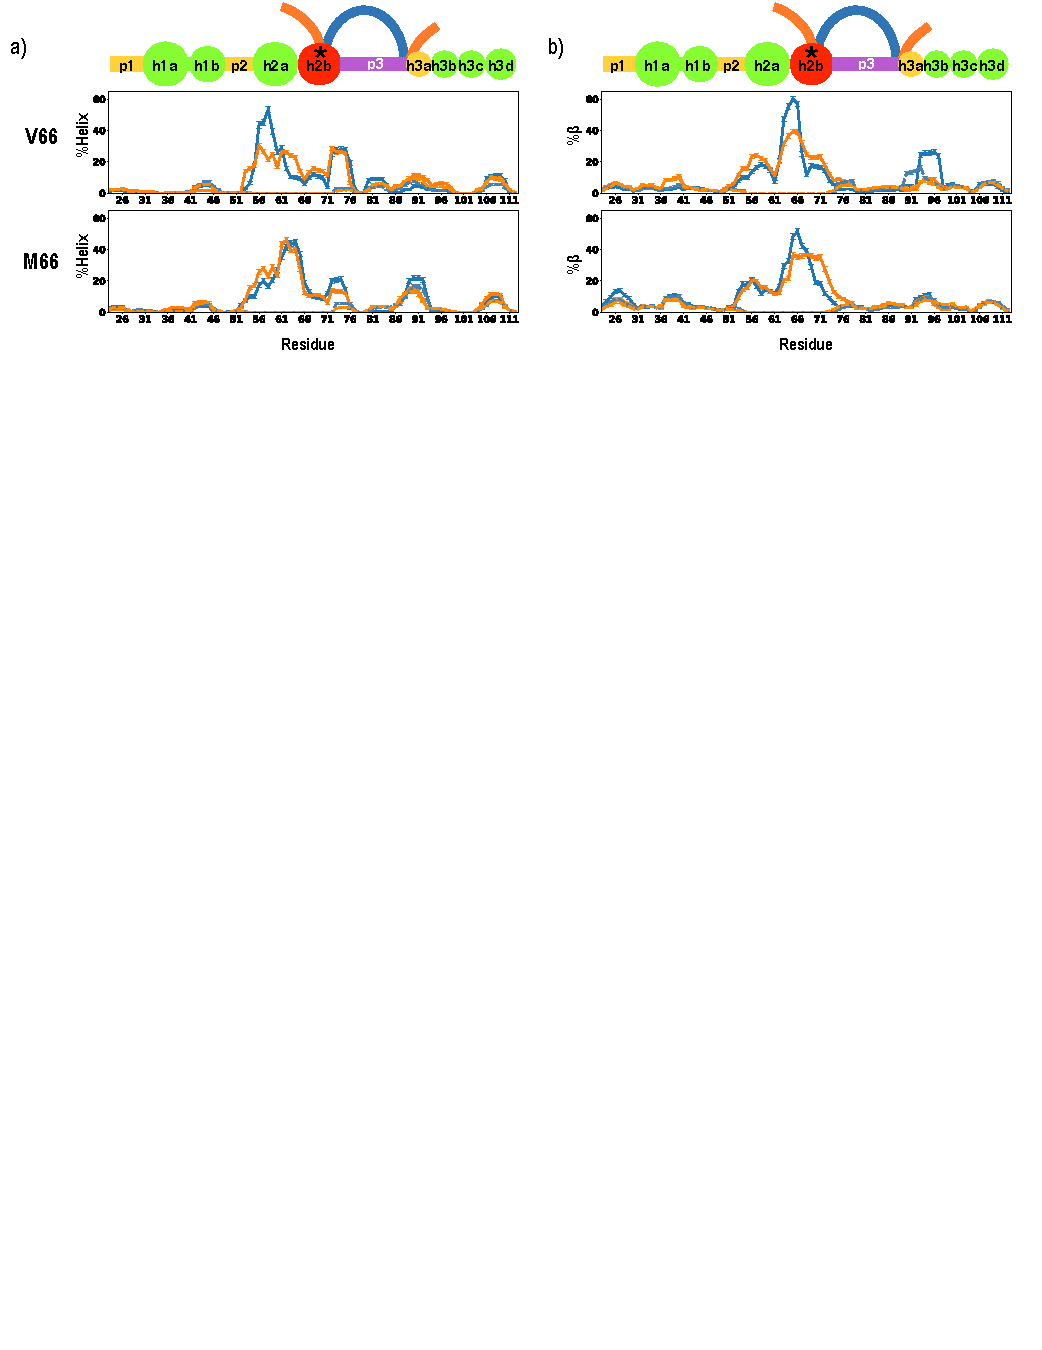
\includegraphics[scale=0.5,width=\textwidth,trim={0 0cm 0 0cm},clip]{../figures/fig6.pdf}
%\caption{{\bf Contributions of each cluster to ensemble of compact, intermediate, and expanded conformations. }
%a) Radius of gyration distribution for entire ensemble is shown for a range of replica temperatures; with the M66 (but not V66) curve revealing at least one high radius of gyration conformation at lower temperatures.  b) Distributions were fit with three gaussian curves of means $\sim1.30nm$ ($\mu$\textsubscript{c}-collapsed), $\sim1.36nm$ ($\mu$\textsubscript{i}-intermediate) and $\sim1.46nm$ ($\mu$\textsubscript{e}-expanded). c) Fit parameters for amplitude of each Gaussian distribution at 300K, revealing a high contribution from the collapsed and expanded states in V66 and M66, respectively. d) Fit amplitudes corresponding to collapsed, expanded and intermediate structures for each cluster at 300K. }
%\label{fig6} 
%\end{figure}

%As shown in Fig~\ref{fig6}d, \nameref{S9_Fig}, \nameref{S10_Fig},
%he collapsed and expanded ensembles are dominated by conformations from cluster BXH and XHB, respectively.  Cluster BXH is split comparably between collapsed and intermediate conformations, while cluster XHB contributes almost exclusively to the amplitude of the expanded conformation. 


% Place figure captions after the first paragraph in which they are cited.



%\subsection*{Tertiary networks in locally disordered clusters can be stabilized or destabilized by salt-bridges }
%\subsection*{Absence of secondary structure at acidic residues local to the SNP increases the ability of these residues to form salt bridges }



%Since the accessibility of these charged side-chains are dependent upon cluster, each cluster has a different salt bridging network.

%Locally ordered clusters (HHH,BBB) have few persistent salt bridges; such conformations have reduced local degrees of freedom and a limited number of local residues that can simultaneously form salt-bridges. Among all clusters, the ordered cluster HHH has the least number of salt bridges and maximum number of hydrogen bonds per frame for both V66 and M66. 

%The disordered clusters BXH and XHB display a large number of salt bridges (Fig~\ref{fig5}c) in similar networks, consistent with important role of electrostatics in maintaining protein disorder. As shown in Fig~\ref{fig7} and \nameref{S11_Fig}, in BXH conformations a high number of salt bridges is associated with a high number of hydrogen bonds, with the most salt-bridges and hydrogen bonds leading to the most compact structures.  In contrast, the hydrogen-bonding pattern of XHB conformations competes with the natural salt-bridging network, so that the number of hydrogen bonds is anti-correlated with the number of salt bridges. This is consistent with the previous characterization by Levine et {\it al}~\cite {Levine2015,Larini2013b}, which demonstrated that increased cooperation between salt bridges and hydrogen bonding resulted in more compact structures even in IDPs. 

%\begin{figure}[!ht]
%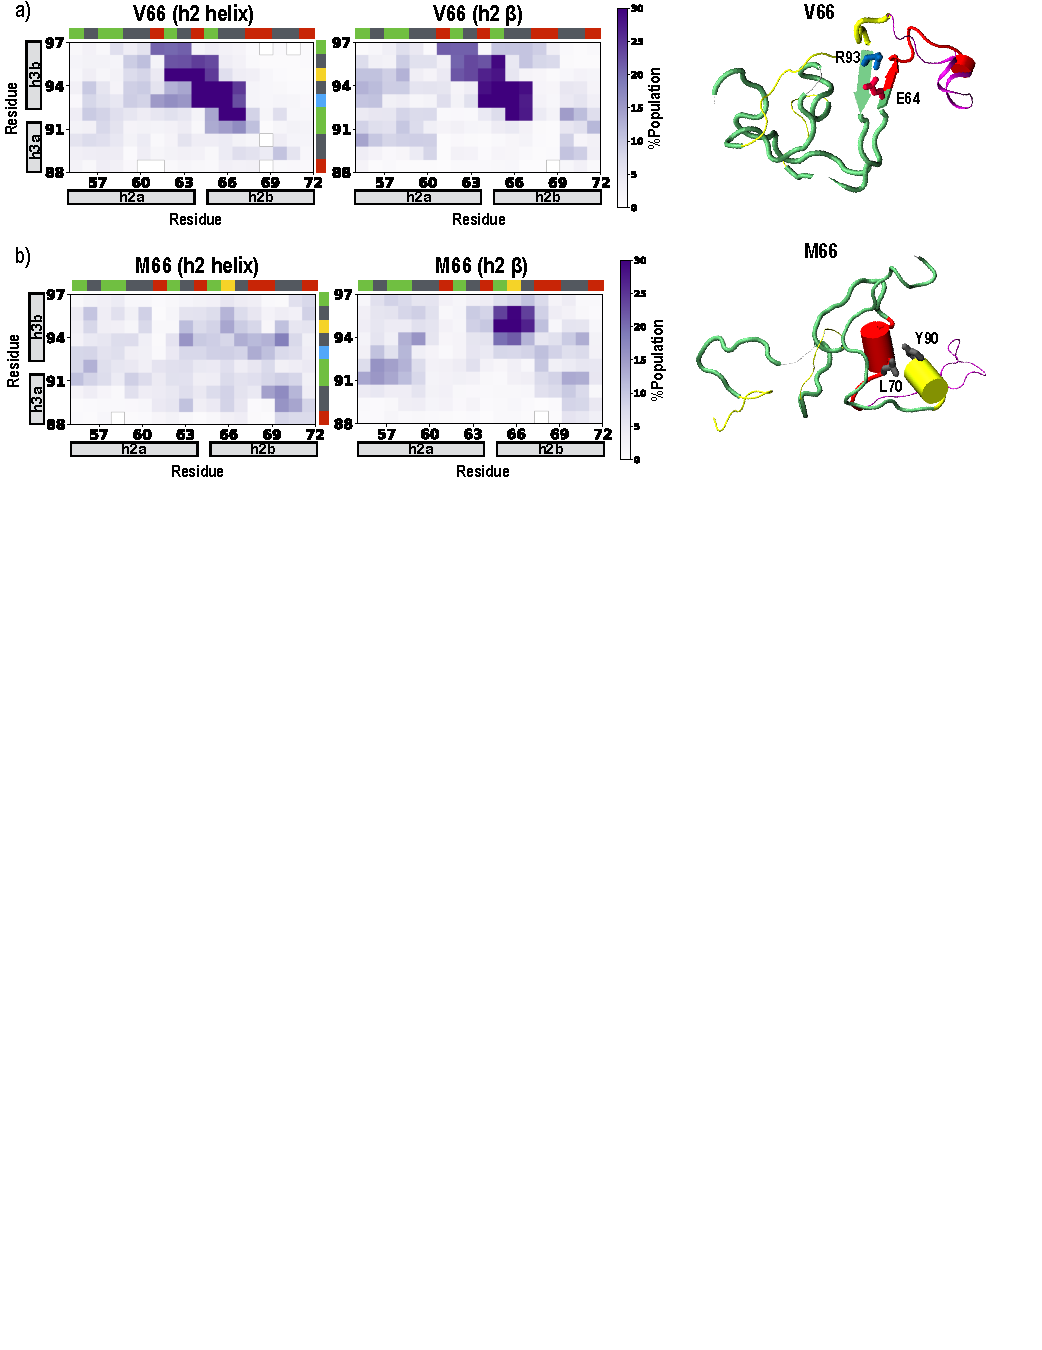
\includegraphics[scale=0.5,width=\textwidth,trim={0 0cm 0 0cm},clip]{../figures/fig7.pdf}
%\caption{{\bf Effects on radius of gyration of switching from cooperation to competition between salt-bridging and hydrogen-bonding.} Binned distributions of the total number of salt bridges, hydrogen-bonds and R\textsubscript{g} for V66 and M66 at low temperatures (300K-317K) 
%Probability densities of the total number of salt bridges per frame vs R\textsubscript{g} or total number of hydrogen bonds per frame for locally-disordered cluster BXH (V66), replaced by cluster XHB for M66. Representative conformations are shown, colored by secondary structure, with residue 66 in orange.}
%\label{fig7} 
%\end{figure}




%In our early efforts to cluster conformations, we intentionally avoided methods that relied too heavily on residue 66, since they seemed likely to artificially exaggerate the effects of the side-chain substitution on long-range interactions.  Despite this concern, clustering based on the peptide backbone at  65,66, and 67 was still eventually selected because it predicted long-range interactions across replicas within a single simulation much more robustly than numerous other methods (and residue combinations).  This clustering method also yields cluster-tertiary contacts relationships that are surprisingly insensitive to side-chain at residue 66 (although cluster populations themselves are affected).



%Shifting this break closer to the sequence midpoint and away from the charge interface (as in cluster XHB), decouples the N-terminal and C-terminal sides and results in an expanded structure in which the N-terminal side is largely ``unfolded.'' (Fig~\ref{fig8})


%The present simulation results identify a compact semi-folded conformation (cluster BXH) which is highly populated for V66 at 300K but uncommon in the M66 ensemble.  The analogous conformation in M66 is cluster XHB, which has a semi-folded C-terminal domain, but an extremely disordered positively-charged N-terminal domain with almost no long-range backbone contacts.  Partial folding or other stabilization of this domain by its interaction with SorCS2 could account for stable M66 binding; it would not be expected for V66, which prefers the enthalpically favorable, more compact BXH cluster even in the unbound state.  



%\textbf{Broader implications} Clustering helps identify different structures within a highly heterogeneous ensemble. The widely used clustering methods (RSMD and dpCA clustering) can observe a large number of clusters due to highly heterogeneous nature of IDPs. Clustering on the basis of dihedral angle of three residues (including the mutation and its immediate neighboring residues), divided the ensemble into five meaningful clusters. This approach of clustering can be widely used on any IDP to characterize its conformational ensemble.
%
%A single point mutation can affect the ensemble through the population of the clusters. Due to weak residue-residue contacts in IDPs, conventional contact maps (residue-residue heat maps) did not provide very much insight. The current method of graphical representation provided us with a meaningful way to characterize tertiary structure of IDPs.

\section*{Materials and Methods}

\subsection*{System setup} To account for differences in starting coil conformation, we included six unique structures to represent residues 23-113 of BDNF prodomain.  All structures were built using I-Tasser ~\cite{Yang2014,Roy2010,Bioinformatics}, Robetta and Modeller ~\cite{Sali1993a}, and all were simulated in a water box at 600K for 50 ns at a constant volume. From the six resulting trajectories, 10 structures with correct proline isomers were selected (based on at least 3ps time interval); in total, our study included 60 unique prodomain structures. All structures were cooled to 300K for 1ns, while prolines were restrained in trans-conformation. M66 replicas were generated by substituting Met for Val at residue 66. Each V66 and M66 replica was placed in a dodecahedron water box with 25,000 TIP3P ~\cite {Jorgensen1983} water molecules and a 0.15M salt concentration (NaCl) for a total system size of approximately 75,000 atoms. The same volume for each replica was ensured by fixing the simulation box of each replica to the average box size (10.2 nm).

\subsubsection*{Molecular Dynamics Simulation} All simulations used the amber99SB-ILDN force field\cite{Lindorff-Larsen} in the GROMACS 5.0.7 simulation package,\cite{Berendsen1995,Abraham2015}, with a time step of 2 fs. 60 replicas were used with temperatures ranging from 300-420K, with exponential spacing. 
Energy minimization for each replica was followed by NVT equilibration at 300K for 1 ns and NPT equilibration at 300K and 1atm pressure for 2ns. 

Each replica was then simulated using T-REMD \cite{Sugita1999a} with an exchange frequency of 1ps for 650 ns, giving a total simulation time of 78 $\mu$s with NVT ensemble. A different random seed was used for the Langevin dynamics of each replica. Long-range electrostatics were calculated using the particle mesh Ewald (PME) method \cite {Essmann1995}, with a 1 nm cutoff and a 0.12 nm grid spacing. Periodic boundary conditions were also used to reduce system size effects. Bonds with H-atoms were constrained using the LINCS (linear constraint solver) algorithm \cite {Hess1997}. The time constant for temperature coupling is 1.5ps. The average exchange acceptance probability ranged between 0.13-0.23 for both V66 and M66. For both V66 and M66 groups, about 500~ns for each replica were discarded for equilibration purposes. 

\subsection*{Analysis of MD Trajectories} For MD simulations, the secondary structure content was  calculated with the STRIDE program incorporated in VMD,\cite{Humphrey1996}  which takes into account the combination of backbone dihedral angles and hydrogen bonding. Helix includes $\alpha$-helix and 3\textsubscript{10}-helix and $\beta$ includes $\beta$-strand and $\beta$-bridge. The hydrogen bonds were calculated with \textbar  D-A\textbar  distance \textless = .35 nm and angle D-H-A angle \textless= 40\textdegree. For salt bridges, distance \textless = .32 nm was used as cutoff between the anionic and cationic atom. The radius of gyration was calculated using the all atoms.

\subsubsection*{Helix length calculation} The length of helix formed at each residue was calculated by determining the number of consecutive residues in which the dihedral angles satisfied $\phi$ \textless 0\textdegree and -120\textdegree\textless $\psi$ \textless 50\textdegree, as in \cite{Nodet,Iglesias2013}.

%\subsubsection*{Clustering} Dihedral angles of residues 65, 66 and 67 at each temperature were used to generate five cluster centroids; these exact values were calculated using K-means clustering algorithm in python. These centroids were used as initial values for k-means algorithm. The ensemble was divided into five clusters at every temperature for both V66 and M66. It was observed that for each cluster, $\psi$ angles were localized within a region noted H (-120\textdegree\textless $\psi$ \textless 50\textdegree, enclosing, but not limited to, the $\alpha-$helix domain of a Ramachandran plot) or B  ($\psi$ \textgreater 50\textdegree or $\psi$ \textless -120\textdegree, enclosing, but not limited to, the $\beta$-sheet region of a Ramachandran plot); the five clusters have been named accordingly, with cluster HHH having residues 65,66, and 67 in the H region for $\sim 99\%$ of its frames, cluster BXH having residue 65 in the B region, no constraints on residue 66, and residue 67 in the H region for $\sim 99\%$ of the frames, etc.
%For the purpose of naming the clusters, the Ramachandran space is divided into two quadrants: H (-120\textdegree\textless $\psi$ \textless 50\textdegree) and B ($\psi$ \textgreater 50\textdegree or $\psi$ \textless -120\textdegree).

%\subsubsection*{Curve fitting for radius of gyration (R\textsubscript{g})} The R\textsubscript{g} distribution curve was fit at each temperature with the sum of three Gaussian functions; these Gaussian functions had means of $\sim1.30nm$ (collapsed), $\sim1.36nm$ (intermediate) and $\sim1.46nm$ (expanded).\begin{equation} y(x) =  A_c.e^{\frac{-(x-\mu_c)^2}{2(\sigma_c)^2}} + A_i.e^{\frac{-(x-\mu_i)^2}{2(\sigma_i)^2}} + A_e.e^{\frac{-(x-\mu_e)^2}{2(\sigma_e)^2}} \end{equation}  where $\mu$\textsubscript{c},$\mu$\textsubscript{i},$\mu$\textsubscript{e} are the means and A\textsubscript{c},A\textsubscript{i},A\textsubscript{e} are the amplitudes for collapsed, intermediate and expanded states respectively.

\subsubsection*{Tertiary contacts network} The contact networks were build using Cytoscape ~\cite {Ahlstrom2013} with linear representation of residues.  Each protein residue comprises a node in the network, with interactions between residues represented as edges. The strength of individual interactions can be interpreted by the  thickness of the edge line on the network diagram. The transparency of an edge increases as it is found at more temperatures.  If residue  66 or its neighboring residues (A51-P79) are involved in h-bond formation, its edge is drawn above the node; otherwise, the edge is drawn at the bottom of the node. To focus on significant interactions, interactions showing more than 3\% persistence were considered in network visualization.      

%\subsubsection*{Interpretation of Chemical Shifts}  Prior to the present study, Anastasia et al\cite{Anastasia2013} measured chemical shifts for the BDNF prodomain (residues 21-113) using NMR, and then used backbone NMR chemical shifts to predict secondary structure via TALOS+ ~\cite{Shen2009} and SSP ~\cite{Marsh2006a}. While TALOS+ has been widely used for structured proteins, neither SSP or TALOS+ differentiates between beta and PPII propensity, which is a significant limitation for disordered proteins.  For comparison with simulation data, we reinterpreted the chemical shifts directly from \cite{Anastasia2013}, deposited at Biological Magnetic Resonance Bank. Secondary structure was predicted using d2D ~\cite{Sormanni2015}, for both chemical shifts (CA,CB,CO,N,HN) generated from MD trajectories using SPARTA+ ~\cite{Shen2010} and the NMR data (This calculation used did not use HA chemical shifts.)  

%\subsubsection*{Identification of Pairing Regions} The regions with peaks in $\beta$ propensity in d2D predictions from NMR data are marked as ``pairing regions'' (Fig~\ref{fig2}c), with region 0\textsuperscript{$\prime$} located at the SNP (residue 66), negatively-notated regions located between the N-terminus and residue 66, and positively-notated regions located between residue 66 and the C-terminus.  


\section*{Acknowledgments}
The authors are grateful to Dr. Clay Bracken and Dr. Barbara Hempstead of Weill Cornell Medical Center for helpful discussions. Computational time was provided through XSEDE resources via NSF MCB110149. 




% Either type in your references using
% \begin{thebibliography}{}
% \bibitem{}
% Text
% \end{thebibliography}
%
% or
%
% Compile your BiBTeX database using our plos2015.bst
% style file and paste the contents of your .bbl file
% here.
\begin{thebibliography}{10}

\bibitem{Uversky2013a}
Uversky VN.
\newblock {Unusual biophysics of intrinsically disordered proteins.}
\newblock Biochim Biophys Acta. 2013;1834(5):932--51.
\newblock doi:{10.1016/j.bbapap.2012.12.008}.

\bibitem{Panchenko2015}
Panchenko AR, Babu MM.
\newblock {Editorial overview: Linking protein sequence and structural changes
  to function in the era of next-generation sequencing}.
\newblock Curr Opin Struct Biol. 2015;32:viii--x.
\newblock doi:{10.1016/j.sbi.2015.06.005}.

\bibitem{Ward2004a}
Ward JJ, Sodhi JS, McGuffin LJ, Buxton BF, Jones DT.
\newblock {Prediction and Functional Analysis of Native Disorder in Proteins
  from the Three Kingdoms of Life}.
\newblock J Mol Biol. 2004;337(3):635--645.
\newblock doi:{10.1016/j.jmb.2004.02.002}.

\bibitem{Dyson2005a}
Dyson HJ, Wright PE.
\newblock {Intrinsically unstructured proteins and their functions}.
\newblock Nat Rev Mol Cell Biol. 2005;6(3):197--208.
\newblock doi:{10.1038/nrm1589}.

\bibitem{Ward2004b}
Ward JJ, Sodhi JS, McGuffin LJ, Buxton BF, Jones DT.
\newblock {Prediction and Functional Analysis of Native Disorder in Proteins
  from the Three Kingdoms of Life}.
\newblock J Mol Biol. 2004;337(3):635--645.
\newblock doi:{10.1016/j.jmb.2004.02.002}.

\bibitem{Dunker2005}
Dunker AK, Cortese MS, Romero P, Iakoucheva LM, Uversky VN.
\newblock {Flexible nets. The roles of intrinsic disorder in protein
  interaction networks}.
\newblock FEBS J. 2005;272(20):5129--5148.
\newblock doi:{10.1111/j.1742-4658.2005.04948.x}.

\bibitem{Habchi2014}
Habchi J, Tompa P, Longhi S, Uversky VN.
\newblock {Introducing Protein Intrinsic Disorder}.
\newblock Chem Rev. 2014;114(13):6561--6588.
\newblock doi:{10.1021/cr400514h}.

\bibitem{Babu2011}
Babu MM, van~der Lee R, de~Groot NS, Gsponer J.
\newblock {Intrinsically disordered proteins: regulation and disease.}
\newblock Curr Opin Struct Biol. 2011;21(3):432--40.
\newblock doi:{10.1016/j.sbi.2011.03.011}.

\bibitem{Sickmeier2007a}
Sickmeier M, Hamilton JA, LeGall T, Vacic V, Cortese MS, Tantos A, et~al.
\newblock {DisProt: the Database of Disordered Proteins}.
\newblock Nucleic Acids Res. 2007;35(Database):D786--D793.
\newblock doi:{10.1093/nar/gkl893}.

\bibitem{Das2015}
Das RK, Ruff KM, Pappu RV.
\newblock {Relating sequence encoded information to form and function of
  intrinsically disordered proteins}.
\newblock Curr Opin Struct Biol. 2015;32:102--112.
\newblock doi:{10.1016/j.sbi.2015.03.008}.

\bibitem{Das2013a}
Das RK, Pappu RV.
\newblock {Conformations of intrinsically disordered proteins are influenced by
  linear sequence distributions of oppositely charged residues.}
\newblock Proc Natl Acad Sci U S A. 2013;110(33):13392--7.
\newblock doi:{10.1073/pnas.1304749110}.

\bibitem{Vacic2012a}
Vacic V, Markwick PRL, Oldfield CJ, Zhao X, Haynes C, Uversky VN, et~al.
\newblock {Disease-associated mutations disrupt functionally important regions
  of intrinsic protein disorder.}
\newblock PLoS Comput Biol. 2012;8(10):e1002709.
\newblock doi:{10.1371/journal.pcbi.1002709}.

\bibitem{Larini2013b}
Larini L, Gessel MM, LaPointe NE, Do TD, Bowers MT, Feinstein SC, et~al.
\newblock {Initiation of assembly of tau(273-284) and its $\Delta$K280 mutant:
  an experimental and computational study}.
\newblock Phys Chem Chem Phys. 2013;15(23):8916.
\newblock doi:{10.1039/c3cp00063j}.

\bibitem{Ganguly2015}
Ganguly D, Chen J, Dyson H, Wright P, Uversky V, Oldfield C, et~al.
\newblock {Modulation of the Disordered Conformational Ensembles of the p53
  Transactivation Domain by Cancer-Associated Mutations}.
\newblock PLOS Comput Biol. 2015;11(4):e1004247.
\newblock doi:{10.1371/journal.pcbi.1004247}.

\bibitem{Viet2014a}
Viet MH, Nguyen PH, Derreumaux P, Li MS.
\newblock {Effect of the English Familial Disease Mutation (H6R) on the
  Monomers and Dimers of A$\beta$40 and A$\beta$42}.
\newblock ACS Chem Neurosci. 2014;5(8):646--657.
\newblock doi:{10.1021/cn500007j}.

\bibitem{Viet2013}
Viet MH, Nguyen PH, Ngo ST, Li MS, Derreumaux P.
\newblock {Effect of the Tottori Familial Disease Mutation (D7N) on the
  Monomers and Dimers of A$\beta$
  {\textless}sub{\textgreater}40{\textless}/sub{\textgreater} and A$\beta$
  {\textless}sub{\textgreater}42{\textless}/sub{\textgreater}}.
\newblock ACS Chem Neurosci. 2013;4(11):1446--1457.
\newblock doi:{10.1021/cn400110d}.

\bibitem{Truong2014a}
Truong PM, Viet MH, Nguyen PH, Hu CK, Li MS.
\newblock {Effect of Taiwan Mutation (D7H) on Structures of Amyloid-$\beta$
  Peptides: Replica Exchange Molecular Dynamics Study}.
\newblock J Phys Chem B. 2014;118(30):8972--8981.
\newblock doi:{10.1021/jp503652s}.

\bibitem{Zhan2013a}
Zhan YA, Wu H, Powell AT, Daughdrill GW, Ytreberg FM.
\newblock {Impact of the K24N mutation on the transactivation domain of p53 and
  its binding to murine double-minute clone 2}.
\newblock Proteins Struct Funct Bioinforma. 2013;81(10):1738--1747.
\newblock doi:{10.1002/prot.24310}.

\bibitem{Xu2013a}
Xu L, Shan S, Wang X.
\newblock {Single Point Mutation Alters the Microstate Dynamics of Amyloid
  $\beta$-Protein A$\beta$42 as Revealed by Dihedral Dynamics Analyses}.
\newblock J Phys Chem B. 2013;117(20):6206--6216.
\newblock doi:{10.1021/jp403288b}.

\bibitem{Bah2016}
Bah A, Forman-Kay JD.
\newblock {Modulation of Intrinsically Disordered Protein Function by
  Post-translational Modifications}.
\newblock J Biol Chem. 2016;291(13):6696--6705.
\newblock doi:{10.1074/jbc.R115.695056}.

\bibitem{He2015}
He Y, Chen Y, Mooney SM, Rajagopalan K, Bhargava A, Sacho E, et~al.
\newblock {Phosphorylation-induced Conformational Ensemble Switching in an
  Intrinsically Disordered Cancer/Testis Antigen}.
\newblock J Biol Chem. 2015;290(41):25090--25102.
\newblock doi:{10.1074/jbc.M115.658583}.

\bibitem{AlexanderConicella2016}
{Alexander Conicella} AE, Zerze GH, Mittal J, {Fawzi Correspondence} NL,
  Conicella AE, Fawzi NL.
\newblock {ALS Mutations Disrupt Phase Separation Mediated by $\alpha$-Helical
  Structure in the TDP-43 Low-Complexity C-Terminal Domain}.
\newblock Struct Des. 2016;24:1537--1549.
\newblock doi:{10.1016/j.str.2016.07.007}.

\bibitem{Iesmantavicius2013}
Ie{\v{s}}mantavi{\v{c}}ius V, Jensen MR, Ozenne V, Blackledge M, Poulsen FM,
  Kjaergaard M.
\newblock {Modulation of the Intrinsic Helix Propensity of an Intrinsically
  Disordered Protein Reveals Long-Range Helix–Helix Interactions}.
\newblock J Am Chem Soc. 2013;135(27):10155--10163.
\newblock doi:{10.1021/ja4045532}.

\bibitem{Mittag2007}
Mittag T, Forman-Kay JD.
\newblock {Atomic-level characterization of disordered protein ensembles}.
\newblock Curr Opin Struct Biol. 2007;17(1):3--14.
\newblock doi:{10.1016/j.sbi.2007.01.009}.

\bibitem{Stanley2015}
Stanley N, Esteban-Mart{\'{i}}n S, {De Fabritiis} G.
\newblock {Progress in studying intrinsically disordered proteins with
  atomistic simulations}.
\newblock Prog Biophys Mol Biol. 2015;119:47--52.
\newblock doi:{10.1016/j.pbiomolbio.2015.03.003}.

\bibitem{Ithuralde2016}
Ithuralde RE, Roitberg AE, Turjanski AG.
\newblock {Structured and Unstructured Binding of an Intrinsically Disordered
  Protein as Revealed by Atomistic Simulations}.
\newblock J Am Chem Soc. 2016;138(28):8742--8751.
\newblock doi:{10.1021/jacs.6b02016}.

\bibitem{Knott2012c}
Knott M, Best RB, Hummer G, de~Bakker P, Word J.
\newblock {A Preformed Binding Interface in the Unbound Ensemble of an
  Intrinsically Disordered Protein: Evidence from Molecular Simulations}.
\newblock PLoS Comput Biol. 2012;8(7):e1002605.
\newblock doi:{10.1371/journal.pcbi.1002605}.

\bibitem{Invernizzi2013}
Invernizzi G, Lambrughi M, Regonesi ME, Tortora P, Papaleo E.
\newblock {The conformational ensemble of the disordered and
  aggregation-protective 182-291 region of ataxin-3.}
\newblock Biochim Biophys Acta. 2013;1830(11):5236--47.
\newblock doi:{10.1016/j.bbagen.2013.07.007}.

\bibitem{Abeln2008}
Abeln S, Frenkel D.
\newblock {Disordered flanks prevent peptide aggregation.}
\newblock PLoS Comput Biol. 2008;4(12):e1000241.
\newblock doi:{10.1371/journal.pcbi.1000241}.

\bibitem{Yedvabny2014}
Yedvabny E, Nerenberg PS, So C, Head-Gordon T.
\newblock {Disordered Structural Ensembles of Vasopressin and Oxytocin and
  Their Mutants}.
\newblock J Phys Chem B. 2015;119(3):896--905.
\newblock doi:{10.1021/jp505902m}.

\bibitem{Levine2015}
Levine ZA, Larini L, LaPointe NE, Feinstein SC, Shea JE.
\newblock {Regulation and aggregation of intrinsically disordered peptides.}
\newblock Proc Natl Acad Sci U S A. 2015;112(9):2758--63.
\newblock doi:{10.1073/pnas.1418155112}.

\bibitem{Pappu2008}
Pappu RV, Wang X, Vitalis A, Crick SL.
\newblock {A polymer physics perspective on driving forces and mechanisms for
  protein aggregation.}
\newblock Arch Biochem Biophys. 2008;469(1):132--41.
\newblock doi:{10.1016/j.abb.2007.08.033}.

\bibitem{Notaras2015}
Notaras M, Hill R, {van den Buuse} M.
\newblock The BDNF gene Val66Met polymorphism as a modifier of psychiatric
  disorder susceptibility: progress and controversy.
\newblock Mol Psychiatry. 2015;20(8):916--930.
\newblock doi:{10.1038/mp.2015.27}.

\bibitem{Korte1995}
Korte M, Carroll P, Wolf E, Brem G, Thoenen H, Bonhoeffer T.
\newblock {Hippocampal long-term potentiation is impaired in mice lacking
  brain-derived neurotrophic factor.}
\newblock Proc Natl Acad Sci. 1995;92(19):8856--8860.
\newblock doi:{10.1073/pnas.92.19.8856}.

\bibitem{Autry2012}
Autry AE, Monteggia LM.
\newblock Brain-derived neurotrophic factor and neuropsychiatric disorders.
\newblock Pharmacol Rev. 2012;64(2):238--258.
\newblock doi:{10.1124/pr.111.005108}.

\bibitem{Bjoerkholm2016}
Bj{\"{o}}rkholm C, Monteggia LM.
\newblock BDNF - a key transducer of antidepressant effects.
\newblock Neuropharmacology. 2016;102:72--79.
\newblock doi:{10.1016/j.neuropharm.2015.10.034}.

\bibitem{Autry2011}
Autry AE, Adachi M, Nosyreva E, Na ES, Los MF, Cheng Pf, et~al.
\newblock NMDA receptor blockade at rest triggers rapid behavioural
  antidepressant responses.
\newblock Nature. 2011;475(7354):91--95.
\newblock doi:{10.1038/nature10130}.

\bibitem{soliman2010}
Soliman F, Glatt CE, Bath KG, Levita L, Jones RM, Pattwell SS, et~al.
\newblock {A genetic variant BDNF polymorphism alters extinction learning in
  both mouse and human.}
\newblock Science. 2010;327(5967):863--6.
\newblock doi:{10.1126/science.1181886}.

\bibitem{Chen2008}
Chen ZY, Bath K, McEwen B, Hempstead B, Lee F.
\newblock {Impact of genetic variant BDNF (Val66Met) on brain structure and
  function.}
\newblock Novartis Found Symp. 2008;289:180--8; discussion 188--95.

\bibitem{Verhagen2010}
Verhagen M, van~der Meij A, van Deurzen PAM, Janzing JGE, Arias-V{\'{a}}squez
  A, Buitelaar JK, et~al.
\newblock {Meta-analysis of the BDNF Val66Met polymorphism in major depressive
  disorder: effects of gender and ethnicity.}
\newblock Mol Psychiatry. 2010;15(3):260--71.
\newblock doi:{10.1038/mp.2008.109}.

\bibitem{Feng2010a}
Feng D, Kim T, {\"{O}}zkan E, Light M, Torkin R, Teng KK, et~al.
\newblock {Molecular and Structural Insight into proNGF Engagement of p75NTR
  and Sortilin}.
\newblock J Mol Biol. 2010;396(4):967--984.
\newblock doi:{10.1016/j.jmb.2009.12.030}.

\bibitem{Anastasia2013}
Anastasia A, Deinhardt K, Chao MV, Will NE, Irmady K, Lee FS, et~al.
\newblock {Val66Met polymorphism of BDNF alters prodomain structure to induce
  neuronal growth cone retraction.}
\newblock Nat Commun. 2013;4:2490.
\newblock doi:{10.1038/ncomms3490}.

\bibitem{Holehouse2017}
Holehouse AS, Das RK, Ahad JN, Richardson MOG, Pappu RV.
\newblock {CIDER: Resources to Analyze Sequence-Ensemble Relationships of
  Intrinsically Disordered Proteins}.
\newblock Biophys J. 2017;112(1):16--21.
\newblock doi:{10.1016/j.bpj.2016.11.3200}.

\bibitem{Yang2014}
Yang J, Yan R, Roy A, Xu D, Poisson J, Zhang Y.
\newblock {The I-TASSER Suite: protein structure and function prediction}.
\newblock Nat Methods. 2014;12(1):7--8.
\newblock doi:{10.1038/nmeth.3213}.

\bibitem{Roy2010}
Roy A, Kucukural A, Zhang Y.
\newblock {I-TASSER: a unified platform for automated protein structure and
  function prediction}.
\newblock Nat Protoc. 2010;5(4):725--738.
\newblock doi:{10.1038/nprot.2010.5}.

\bibitem{Bioinformatics}
Zhang Y.
\newblock {I-TASSER server for protein 3D structure prediction}.
\newblock BMC Bioinformatics. 2008;9(1):40.
\newblock doi:{10.1186/1471-2105-9-40}.

\bibitem{Sali1993a}
{\v{S}}ali A, Blundell TL.
\newblock {Comparative Protein Modelling by Satisfaction of Spatial
  Restraints}.
\newblock J Mol Biol. 1993;234(3):779--815.
\newblock doi:{10.1006/jmbi.1993.1626}.

\bibitem{Jorgensen1983}
Jorgensen WL, Chandrasekhar J, Madura JD, Impey RW, Klein ML.
\newblock {Comparison of simple potential functions for simulating liquid
  water}.
\newblock J Chem Phys. 1983;79(2):926--935.
\newblock doi:{10.1063/1.445869}.

\bibitem{Lindorff-Larsen}
Lindorff-Larsen K, Piana S, Palmo K, Maragakis P, Klepeis JL, Dror RO, et~al.
\newblock {Improved side-chain torsion potentials for the Amber ff99SB protein
  force field}.
\newblock Proteins Struct Funct Bioinforma. 2010; p. NA--NA.
\newblock doi:{10.1002/prot.22711}.

\bibitem{Berendsen1995}
Berendsen HJC, van~der Spoel D, van Drunen R.
\newblock {GROMACS: A message-passing parallel molecular dynamics
  implementation}.
\newblock Comput Phys Commun. 1995;91(1-3):43--56.
\newblock doi:{10.1016/0010-4655(95)00042-E}.

\bibitem{Abraham2015}
Abraham MJ, Murtola T, Schulz R, P{\'{a}}ll S, Smith JC, Hess B, et~al.
\newblock {Gromacs: High performance molecular simulations through multi-level
  parallelism from laptops to supercomputers}.
\newblock SoftwareX. 2015;1-2(June 2016):19--25.
\newblock doi:{10.1016/j.softx.2015.06.001}.

\bibitem{Sugita1999a}
Sugita Y, Okamoto Y.
\newblock {Replica-exchange molecular dynamics method for protein folding}.
\newblock Chem Phys Lett. 1999;314(1-2):141--151.
\newblock doi:{10.1016/S0009-2614(99)01123-9}.

\bibitem{Essmann1995}
Essmann U, Perera L, Berkowitz ML, Darden T, Lee H, Pedersen LG.
\newblock {A smooth particle mesh Ewald method}.
\newblock J Chem Phys. 1995;103(19):8577--8593.
\newblock doi:{10.1063/1.470117}.

\bibitem{Hess1997}
Hess B, Bekker H, Berendsen HJC, Fraaije JGEM.
\newblock {LINCS: A linear constraint solver for molecular simulations}.
\newblock J Comput Chem. 1997;18(12):1463--1472.
\newblock doi:{10.1002/(SICI)1096-987X(199709)18:12\textless1463::AID-JCC4\textgreater3.0.CO;2-H}.

\bibitem{Humphrey1996}
Humphrey W, Dalke A, Schulten K.
\newblock {VMD: visual molecular dynamics.}
\newblock J Mol Graph. 1996;14(1):33--8, 27--8.

\bibitem{Nodet}
Nodet G, Salmon L, Ozenne V, Meier S, Jensen MR, Blackledge M.
\newblock {Quantitative Description of Backbone Conformational Sampling of
  Unfolded Proteins at Amino Acid Resolution from NMR Residual Dipolar
  Couplings}.
\newblock J Am Chem Soc. 2009;131(49):17908--17918.
\newblock doi:{10.1021/ja9069024}.

\bibitem{Iglesias2013}
Iglesias J, Sanchez-Mart{\'{i}}nez M, Crehuet R.
\newblock {SS-map}.
\newblock Intrinsically Disord Proteins. 2013;1(1):e25323.
\newblock doi:{10.4161/idp.25323}.

\bibitem{Ahlstrom2013}
Ahlstrom LS, Baker JL, Ehrlich K, Campbell ZT, Patel S, Vorontsov II, et~al.
\newblock {Network visualization of conformational sampling during molecular
  dynamics simulation.}
\newblock J Mol Graph Model. 2013;46:140--9.
\newblock doi:{10.1016/j.jmgm.2013.10.003}.

\bibitem{Shen2009}
Shen Y, Delaglio F, Cornilescu G, Bax A.
\newblock {TALOS+: a hybrid method for predicting protein backbone torsion
  angles from NMR chemical shifts.}
\newblock J Biomol NMR. 2009;44(4):213--23.
\newblock doi:{10.1007/s10858-009-9333-z}.

\bibitem{Marsh2006a}
Marsh JA, Singh VK, Jia Z, Forman-Kay JD.
\newblock {Sensitivity of secondary structure propensities to sequence
  differences between $\alpha$- and $\gamma$-synuclein: Implications for
  fibrillation}.
\newblock Protein Sci. 2006;15(12):2795--2804.
\newblock doi:{10.1110/ps.062465306}.

\bibitem{Sormanni2015}
Sormanni P, Camilloni C, Fariselli P, Vendruscolo M.
\newblock {The s2D Method: Simultaneous Sequence-Based Prediction of the
  Statistical Populations of Ordered and Disordered Regions in Proteins}.
\newblock J Mol Biol. 2015;427(4):982--996.
\newblock doi:{10.1016/j.jmb.2014.12.007}.

\bibitem{Shen2010}
Shen Y, Bax A.
\newblock {SPARTA+: a modest improvement in empirical NMR chemical shift
  prediction by means of an artificial neural network}.
\newblock J Biomol NMR. 2010;48(1):13--22.
\newblock doi:{10.1007/s10858-010-9433-9}.

\bibitem{Creamer1992}
Creamer TP, Rose GD.
\newblock {Side-chain entropy opposes a-helix formation but rationalizes
  experimentally determined helix-forming propensities (a-helix/protein
  folding/protein engineering)}.
\newblock Nat Sci. 1992;89(250):5937--5941.

\end{thebibliography}


%\bibliography{../IDP_Val66Met_Lohia/idp_ref,BDNF_2016}

\section*{Supporting Information}

\paragraph*{S1 Fig.}
\label{S1_Fig}
{\bf Mixing of replicas during the simulation.}
a) Mean square displacement (MSD) of each replica in the temperature range (300K-420K) for both V66 and M66. Replicas visiting 300K are colored green and remaining replicas are colored red. b) Population of each replica at 300K. c) Number of round trips completed by each replica.

\paragraph*{S2 Fig.}
\label{S2_Fig} 
{\bf Temperature dependence of helical length around residue 66. }
a) Helical propensity at residues 50-77, determined from STRIDE, for helix of length 10,11 and 12 containing residue 66, with curves colored according to temperature. M66 folds into a 12 residue helix at residues 62-74 at high temperature. Representative conformations are shown, colored by secondary structure, with residue 66 in stick representation. b) Total number of replicas at which lengths for helices containing residue 66 is observed, for a range of temperatures. The helices of longer lengths are formed in 4 or more replicas at high temperatures. 

\paragraph*{S3 Fig.}
\label{S3_Fig} 
{\bf Backbone hydrogen bonding partners of residue 66 and length of beta sheet formed at every residue at 300K .}
a) Population of backbone hydrogen bonding of residue 66 with all other residues in the sequence. Residue 66 forms a weak contact with residue at +4\textsuperscript{$\prime$} region b) Length of beta strands formed at each residue. Pairing regions show higher density of beta of length 3 or more for both V66 and M66. The strand length formed at each residue was calculated by determining the number of consecutive residues in which the dihedral angles satisfied $\psi$ \textgreater 50\textdegree and $\phi$ \textless -90\textdegree  or $\psi$ \textless -120\textdegree and $\phi$ \textless -90\textdegree.

\paragraph*{S4 Fig.}
\label{S4_Fig} 
{\bf Distribution of dihedral angles at residue 65,66 and 67 for each cluster at 300K.}

\paragraph*{S5 Fig.}
\label{S5_Fig} 
{\bf Distribution of dihedral angles with temperature at residue 65,66 and 67 at each cluster.}
Dotted lines correspond to  -120\textdegree \textless  $\psi$ \textless  50\textdegree. 

\paragraph*{S6 Fig.}
\label{S6_Fig} 
{\bf Linear networks of transient tertiary contacts} a) Hydrogen-bonding and b) salt-bridging pairs are shown for the entire ensemble and then decomposed by cluster at high temperatures (398K-420K). The backbone tertiary-contact network is made for V66 and M66, with each residue serving as a node in the network, as described in Methods. Residues at the pairing regions  
are colored black. Backbone interactions serve as edges between individual network nodes; the thickness of the edge corresponds to the strength of the hydrogen bond, and the transparency of the edge increases as its frequency increases. If residue 66 or its nearby residues (A51-P79) are involved in hydrogen-bond formation then the edge is drawn above the node; otherwise, it is drawn at the bottom of the node. Fewer contact pairs are observed at high temperatures. V66 forms stronger backbone hydrogen-bonding for beta bridge formations and M66 forms stronger backbone hydrogen-bonding for helix formation at residue 66. Cluster HHH in M66 simultaneously forms salt-bridge and hydrogen bonds from residues near the SNP. 

\paragraph*{S7 Fig.}
\label{S7_Fig} 
{\bf Secondary structure propensity, determined using STRIDE from MD trajectories, at each residue, with curves colored according to temperature.}

\paragraph*{S8 Fig.}
\label{S8_Fig} 
{\bf Length of helix formed at every cluster at 300K.} Cluster HHH and Cluster XHB can form long cooperative helices at residue 66. A Smaller helix with 8 or fewer residues forms near residue 66 for clusters BXH,BBB and HBB.
 
\paragraph*{S9 Fig.}
\label{S9_Fig} 
{\bf Distribution of R\textsubscript{g} for each cluster.}
\textless R\textsubscript{g}\textgreater with temperature for a) entire ensemble and b) each cluster. The \textless R\textsubscript{g}\textgreater for V66 and M66 reverses with increase in temperature. We observe the same trend reversal for cluster HHH. c) Distribution of R\textsubscript{g} for each cluster at every temperature. The line color transitions from blue (cold) to red (hot) with increase in temperature from 300K to 420K. 

\paragraph*{S10 Fig.}
\label{S10_Fig} 
{\bf Distribution of amplitude of the fitted gaussian curves with temperature.}
Cluster BXH and XHB shows high amplitude of collapsed and expanded states, respectively at 300K. Cluster HHH shows increase in amplitude for collapsed structure at high temperature.

\paragraph*{S11 Fig.}
\label{S11_Fig} 
{\bf Population densities of salt bridges and hydrogen bonds for V66 and M66 for each cluster at low temperatures (300K-317K).}
Simultaneous salt bridge and hydrogen bonds formation stabilize cluster BXH and only salt bridge formation destabilize cluster XHB.  a) Population densities of total number of salt bridges per frame vs R\textsubscript{g} (normalized with respect to total number of frames). b) Population densities of total number of hydrogen bonds per frame vs R\textsubscript{g} (normalized with respect to total number of frames). c) Population densities of total number of salt bridge per frame vs total number of hydrogen bonds  per frame ( normalized with respect to total number of frames).



\end{document}

